%%
%% This is file `sample-sigconf-authordraft.tex',
%% generated with the docstrip utility.
%%
%% The original source files were:
%%
%% samples.dtx  (with options: `all,proceedings,bibtex,authordraft')
%% 
%% IMPORTANT NOTICE:
%% 
%% For the copyright see the source file.
%% 
%% Any modified versions of this file must be renamed
%% with new filenames distinct from sample-sigconf-authordraft.tex.
%% 
%% For distribution of the original source see the terms
%% for copying and modification in the file samples.dtx.
%% 
%% This generated file may be distributed as long as the
%% original source files, as listed above, are part of the
%% same distribution. (The sources need not necessarily be
%% in the same archive or directory.)
%%
%%
%% Commands for TeXCount
%TC:macro \cite [option:text,text]
%TC:macro \citep [option:text,text]
%TC:macro \citet [option:text,text]
%TC:envir table 0 1
%TC:envir table* 0 1
%TC:envir tabular [ignore] word
%TC:envir displaymath 0 word
%TC:envir math 0 word
%TC:envir comment 0 0
%%
%%
%% The first command in your LaTeX source must be the \documentclass
%% command.
%%
%% For submission and review of your manuscript please change the
%% command to \documentclass[manuscript, screen, review]{acmart}.
%%
%% When submitting camera ready or to TAPS, please change the command
%\documentclass[sigconf]{acmart} 
%or whichever template is required
%% for your publication.
%%
%%
\documentclass[sigconf,nonacm,timestamp]{acmart}
%\documentclass[manuscript,screen,review,anonymous]{acmart}
%\settopmatter{printacmref=false, printccs=true, printfolios=true}


%%
%% \BibTeX command to typeset BibTeX logo in the docs
\AtBeginDocument{%
  \providecommand\BibTeX{{%
    Bib\TeX}}}

%% Rights management information.  This information is sent to you
%% when you complete the rights form.  These commands have SAMPLE
%% values in them; it is your responsibility as an author to replace
%% the commands and values with those provided to you when you
%% complete the rights form.
\setcopyright{acmlicensed}
\copyrightyear{2025}
\acmYear{2025}
\acmDOI{XXXXXXX.XXXXXXX}

%% These commands are for a PROCEEDINGS abstract or paper.
\acmConference[ACM CUI 2025]{ACM CUI 2025}{July 8,
  2025}{Waterloo, Ontario, Canada}
%%
%%  Uncomment \acmBooktitle if the title of the proceedings is different
%%  from ``Proceedings of ...''!
%%
%%\acmBooktitle{Woodstock '18: ACM Symposium on Neural Gaze Detection,
%%  June 03--05, 2018, Woodstock, NY}
\acmISBN{978-1-4503-XXXX-X/18/06}


%%
%% Submission ID.
%% Use this when submitting an article to a sponsored event. You'll
%% receive a unique submission ID from the organizers
%% of the event, and this ID should be used as the parameter to this command.
%%\acmSubmissionID{123-A56-BU3}

%%
%% For managing citations, it is recommended to use bibliography
%% files in BibTeX format.
%%
%% You can then either use BibTeX with the ACM-Reference-Format style,
%% or BibLaTeX with the acmnumeric or acmauthoryear sytles, that include
%% support for advanced citation of software artefact from the
%% biblatex-software package, also separately available on CTAN.
%%
%% Look at the sample-*-biblatex.tex files for templates showcasing
%% the biblatex styles.
%%

%%
%% The majority of ACM publications use numbered citations and
%% references.  The command \citestyle{authoryear} switches to the
%% "author year" style.
%%
%% If you are preparing content for an event
%% sponsored by ACM SIGGRAPH, you must use the "author year" style of
%% citations and references.
%% Uncommenting
%% the next command will enable that style.
%%\citestyle{acmauthoryear}

\usepackage{tabularx}
\usepackage{adjustbox}
\usepackage{geometry}
\usepackage{enumitem}
\usepackage{tcolorbox}
\usepackage{amsmath}
\usepackage{multicol}
\usepackage{svg}
\usepackage{tikz, pgfplots}
\pgfplotsset{compat=1.18}
\usepackage{subcaption}
\usetikzlibrary{matrix}
\usepackage{xcolor}
\definecolor{gray(x11gray)}{rgb}{0.75, 0.75, 0.75}

%%
%% end of the preamble, start of the body of the document source.
\begin{document}

%%
%% The "title" command has an optional parameter,
%% allowing the author to define a "short title" to be used in page headers.

\title{Static Vs. Agentic Game Master AI for Facilitating Solo Role-Playing Experiences}

%\title{Game Master AI: ReAct Prompting for Dynamic RPG Narratives}

%\title{When friends are rare: Enabling Conversational Interactive Fiction and Tabletop Role Playing with AI}

%%
%% The "author" command and its associated commands are used to define
%% the authors and their affiliations.
%% Of note is the shared affiliation of the first two authors, and the
%% "authornote" and "authornotemark" commands
%% used to denote shared contribution to the research.
\author{Nicolai H. J{\o}rgensen}
%\authornote{Both authors contributed equally to this research.}
\affiliation{%
  \institution{Department of Computer Science, Aalborg University}
  \city{Aalborg}
  \country{Denmark}
}
\email{njarge20@student.aau.dk}

\author{Sarmilan Tharmabalan}
%\authornotemark[1]
\affiliation{%
  \institution{Department of Computer Science, Aalborg University}
  \city{Aalborg}
  \country{Denmark}
}
\email{stharm20@student.aau.dk}

\author{Ilhan Aslan}
%\authornotemark[1]
\affiliation{%
  \institution{Department of Computer Science, Aalborg University}
  \city{Aalborg}
  \country{Denmark}
}
\email{ilas@cs.aau.dk}

\author{Nicolai Brodersen Hansen}
%\authornotemark[1]
\affiliation{%
  \institution{Department of Computer Science, Aalborg University}
  \city{Aalborg}
  \country{Denmark}
}
\email{nbha@cs.aau.dk}

\author{Timothy Merritt}
%\authornotemark[1]
\affiliation{%
  \institution{Department of Computer Science, Aalborg University}
  \city{Aalborg}
  \country{Denmark}
}
\email{merritt@cs.aau.dk}

%\author{Timothy R. Merritt}
%\orcid{0000-0002-7851-7339}
%\affiliation{%
%  \institution{Department of Computer Science, Aalborg University}
%  \city{Aalborg}
%  \country{Denmark}
%}
%\email{merritt@cs.aau.dk}


%%
%% By default, the full list of authors will be used in the page
%% headers. Often, this list is too long, and will overlap
%% other information printed in the page headers. This command allows
%% the author to define a more concise list
%% of authors' names for this purpose.
\renewcommand{\shortauthors}{J{\o}rgensen et al.}

%%
%% The abstract is a short summary of the work to be presented in the
%% article.
\begin{abstract}
%This paper presents a sophisticated multi-agent system designed to enhance interactive narrative experiences in single-player role-playing games, specifically addressing the limitations of solo engagement in tabletop games like Dungeons \& Dragons. Building upon the foundation laid by our previous work on ChatRPG, an AI-driven text-based role-playing game, we introduce a new version utilizing the ReAct framework. This enhanced system comprises two ReAct agents: the \textbf{Narrator}, responsible for generating immersive narratives, and the \textbf{Archivist}, which manages memory and context. Our approach significantly improves the system’s upgradability and extensibility, allowing for seamless integration of advanced features such as multimedia content and enhanced storytelling in future research. Comparative studies between the original and the upgraded systems demonstrate not only maintained performance but also superior user engagement with the latter. This research sets the stage for further exploration into how interactive fiction can be revolutionized through AI advancements, offering a richer and more immersive gaming experience for solo players. The paper details the design and evaluation process, providing insights for future enhancements in AI-driven role-playing games.

%This paper presents an advanced multi-agent system designed to enhance interactive narratives in single-player role-playing games, addressing the limitations of solo engagement in tabletop experiences like Dungeons \& Dragons. We introduce an AI-driven text-based role-playing system leveraging the ReAct framework to include reasoning and action, which builds on a previous system using simplified prompt engineering. Our system integrates two ReAct agents: the Narrator, which generates immersive narratives, and the Archivist, which manages memory and context. This architecture enhances modularity, facilitating future integration of multimedia content and advanced storytelling features. Comparative evaluations demonstrate that the agentic system maintains performance while significantly improving user engagement. Our findings contribute to the evolution of AI-driven interactive fiction, highlighting new avenues for enhancing solo role-playing experiences.

%
This paper presents a game master AI for single-player role-playing games. The AI is designed to deliver interactive text-based narratives and experiences typically associated with multiplayer tabletop games like Dungeons \& Dragons. We report on the design process and the series of experiments to improve the functionality and experience design, resulting in two functional versions of the system.
While v1 of our system uses simplified prompt engineering, v2 leverages a multi-agent architecture and the ReAct framework to include reasoning and action. A comparative evaluation demonstrates that v2 as an agentic system maintains play while significantly improving modularity and game experience, including immersion and curiosity. Our findings contribute to the evolution of AI-driven interactive fiction, highlighting new avenues for enhancing solo role-playing experiences.



\end{abstract}

%%
%% The code below is generated by the tool at http://dl.acm.org/ccs.cfm.
%% Please copy and paste the code instead of the example below.
%%
\begin{CCSXML}
<ccs2012>
   <concept>
       <concept_id>10010147.10010178.10010179.10010182</concept_id>
       <concept_desc>Computing methodologies~Natural language generation</concept_desc>
       <concept_significance>500</concept_significance>
       </concept>
   <concept>
       <concept_id>10010147.10010178.10010219.10010220</concept_id>
       <concept_desc>Computing methodologies~Multi-agent systems</concept_desc>
       <concept_significance>500</concept_significance>
       </concept>
 </ccs2012>
\end{CCSXML}

\ccsdesc[500]{Computing methodologies~Natural language generation}
\ccsdesc[500]{Computing methodologies~Multi-agent systems}

%%
%% Keywords. The author(s) should pick words that accurately describe
%% the work being presented. Separate the keywords with commas.
\keywords{Interactive Fiction, Role-Playing Games, Dungeons \& Dragons, User Engagement, AI Game Master, ReAct, LangChain, Large Language Models, Multi-Agent System, Generative AI}
%% A "teaser" image appears between the author and affiliation
%% information and the body of the document, and typically spans the
%% page.
%\begin{teaserfigure}
%  \includegraphics[width=\textwidth]{sampleteaser}
%  \caption{Seattle Mariners at Spring Training, 2010.}
%  \Description{Enjoying the baseball game from the third-base
%  seats. Ichiro Suzuki preparing to bat.}
%  \label{fig:teaser}
%\end{teaserfigure}

\begin{teaserfigure}
  \includegraphics[width=\textwidth]{0_pictures/agenticGM_teaser.JPG}
  \caption{Conceptual image of the vision behind ChatRPG. The player at the left uses the text-based chat user interface of the role-playing game to explore and respond to the game events and take actions in the game. The Game Master AI (GM AI) builds an engaging narrative, communicates details about the fictional world, and manages the assets, events, and status to maintain coherence.}
  \Description{A conceptual image showing the vision behind ChatRPG. On the left a player is shown looking at a screen and typing text. Behind the screen is the Game Master AI depicted. One aspect of the Game Master is narrating the story to the player, while another aspect is retrieving and storing information from a shelf of books.}
  \label{fig:teaser}
\end{teaserfigure}


%\received{20 February 2007}
%\received[revised]{12 March 2009}
%\received[accepted]{5 June 2009}

%%
%% This command processes the author and affiliation and title
%% information and builds the first part of the formatted document.
\maketitle





\section{Introduction}

Video generation has garnered significant attention owing to its transformative potential across a wide range of applications, such media content creation~\citep{polyak2024movie}, advertising~\citep{zhang2024virbo,bacher2021advert}, video games~\citep{yang2024playable,valevski2024diffusion, oasis2024}, and world model simulators~\citep{ha2018world, videoworldsimulators2024, agarwal2025cosmos}. Benefiting from advanced generative algorithms~\citep{goodfellow2014generative, ho2020denoising, liu2023flow, lipman2023flow}, scalable model architectures~\citep{vaswani2017attention, peebles2023scalable}, vast amounts of internet-sourced data~\citep{chen2024panda, nan2024openvid, ju2024miradata}, and ongoing expansion of computing capabilities~\citep{nvidia2022h100, nvidia2023dgxgh200, nvidia2024h200nvl}, remarkable advancements have been achieved in the field of video generation~\citep{ho2022video, ho2022imagen, singer2023makeavideo, blattmann2023align, videoworldsimulators2024, kuaishou2024klingai, yang2024cogvideox, jin2024pyramidal, polyak2024movie, kong2024hunyuanvideo, ji2024prompt}.


In this work, we present \textbf{\ours}, a family of rectified flow~\citep{lipman2023flow, liu2023flow} transformer models designed for joint image and video generation, establishing a pathway toward industry-grade performance. This report centers on four key components: data curation, model architecture design, flow formulation, and training infrastructure optimization—each rigorously refined to meet the demands of high-quality, large-scale video generation.


\begin{figure}[ht]
    \centering
    \begin{subfigure}[b]{0.82\linewidth}
        \centering
        \includegraphics[width=\linewidth]{figures/t2i_1024.pdf}
        \caption{Text-to-Image Samples}\label{fig:main-demo-t2i}
    \end{subfigure}
    \vfill
    \begin{subfigure}[b]{0.82\linewidth}
        \centering
        \includegraphics[width=\linewidth]{figures/t2v_samples.pdf}
        \caption{Text-to-Video Samples}\label{fig:main-demo-t2v}
    \end{subfigure}
\caption{\textbf{Generated samples from \ours.} Key components are highlighted in \textcolor{red}{\textbf{RED}}.}\label{fig:main-demo}
\end{figure}


First, we present a comprehensive data processing pipeline designed to construct large-scale, high-quality image and video-text datasets. The pipeline integrates multiple advanced techniques, including video and image filtering based on aesthetic scores, OCR-driven content analysis, and subjective evaluations, to ensure exceptional visual and contextual quality. Furthermore, we employ multimodal large language models~(MLLMs)~\citep{yuan2025tarsier2} to generate dense and contextually aligned captions, which are subsequently refined using an additional large language model~(LLM)~\citep{yang2024qwen2} to enhance their accuracy, fluency, and descriptive richness. As a result, we have curated a robust training dataset comprising approximately 36M video-text pairs and 160M image-text pairs, which are proven sufficient for training industry-level generative models.

Secondly, we take a pioneering step by applying rectified flow formulation~\citep{lipman2023flow} for joint image and video generation, implemented through the \ours model family, which comprises Transformer architectures with 2B and 8B parameters. At its core, the \ours framework employs a 3D joint image-video variational autoencoder (VAE) to compress image and video inputs into a shared latent space, facilitating unified representation. This shared latent space is coupled with a full-attention~\citep{vaswani2017attention} mechanism, enabling seamless joint training of image and video. This architecture delivers high-quality, coherent outputs across both images and videos, establishing a unified framework for visual generation tasks.


Furthermore, to support the training of \ours at scale, we have developed a robust infrastructure tailored for large-scale model training. Our approach incorporates advanced parallelism strategies~\citep{jacobs2023deepspeed, pytorch_fsdp} to manage memory efficiently during long-context training. Additionally, we employ ByteCheckpoint~\citep{wan2024bytecheckpoint} for high-performance checkpointing and integrate fault-tolerant mechanisms from MegaScale~\citep{jiang2024megascale} to ensure stability and scalability across large GPU clusters. These optimizations enable \ours to handle the computational and data challenges of generative modeling with exceptional efficiency and reliability.


We evaluate \ours on both text-to-image and text-to-video benchmarks to highlight its competitive advantages. For text-to-image generation, \ours-T2I demonstrates strong performance across multiple benchmarks, including T2I-CompBench~\citep{huang2023t2i-compbench}, GenEval~\citep{ghosh2024geneval}, and DPG-Bench~\citep{hu2024ella_dbgbench}, excelling in both visual quality and text-image alignment. In text-to-video benchmarks, \ours-T2V achieves state-of-the-art performance on the UCF-101~\citep{ucf101} zero-shot generation task. Additionally, \ours-T2V attains an impressive score of \textbf{84.85} on VBench~\citep{huang2024vbench}, securing the top position on the leaderboard (as of 2025-01-25) and surpassing several leading commercial text-to-video models. Qualitative results, illustrated in \Cref{fig:main-demo}, further demonstrate the superior quality of the generated media samples. These findings underscore \ours's effectiveness in multi-modal generation and its potential as a high-performing solution for both research and commercial applications.

\section{Background} \label{section:LLM}

% \subsection{Large Language Model (LLM)}   

Figure~\ref{fig:LLaMA_model}(a) shows that a decoder-only LLM initially processes a user prompt in the “prefill” stage and subsequently generates tokens sequentially during the “decoding” stage.
Both stages contain an input embedding layer, multiple decoder transformer blocks, an output embedding layer, and a sampling layer.
Figure~\ref{fig:LLaMA_model}(b) demonstrates that the decoder transformer blocks consist of a self attention and a feed-forward network (FFN) layer, each paired with residual connection and normalization layers. 

% Differentiate between encoder/decoder, explain why operation intensity is low, explain the different parts of a transformer block. Discuss Table II here. 

% Explain the architecture with Llama2-70B.

% \begin{table}[thb]
% \renewcommand\arraystretch{1.05}
% \centering
% % \vspace{-5mm}
%     \caption{ML Model Parameter Size and Operational Intensity}
%     \vspace{-2mm}
%     \small
%     \label{tab:ML Model Parameter Size and Operational Intensity}    
%     \scalebox{0.95}{
%         \begin{tabular}{|c|c|c|c|c|}
%             \hline
%             & Llama2 & BLOOM & BERT & ResNet \\
%             Model & (70B) & (176B) & & 152 \\
%             \hline
%             Parameter Size (GB) & 140 & 352 & 0.17 & 0.16 \\
%             \hline
%             Op Intensity (Ops/Byte) & 1 & 1 & 282 & 346 \\
%             \hline
%           \end{tabular}
%     }
% \vspace{-3mm}
% \end{table}

% {\fontsize{8pt}{11pt}\selectfont 8pt font size test Memory Requirement}

\begin{figure}[t]
    \centering
    \includegraphics[width=8cm]{Figure/LLaMA_model_new_new.pdf}
    \caption{(a) Prefill stage encodes prompt tokens in parallel. Decoding stage generates output tokens sequentially.
    (b) LLM contains N$\times$ decoder transformer blocks. 
    (c) Llama2 model architecture.}
    \label{fig:LLaMA_model}
\end{figure}

Figure~\ref{fig:LLaMA_model}(c) demonstrates the Llama2~\cite{touvron2023llama} model architecture as a representative LLM.
% The self attention layer requires three GEMVs\footnote{GEMVs in multi-head attention~\cite{attention}, narrow GEMMs in grouped-query attention~\cite{gqa}.} to generate query, key and value vectors.
In the self-attention layer, query, key and value vectors are generated by multiplying input vector to corresponding weight matrices.
These matrices are segmented into multiple heads, representing different semantic dimensions.
The query and key vectors go though Rotary Positional Embedding (RoPE) to encode the relative positional information~\cite{rope-paper}.
Within each head, the generated key and value vectors are appended to their caches.
The query vector is multiplied by the key cache to produce a score vector.
After the Softmax operation, the score vector is multiplied by the value cache to yield the output vector.
The output vectors from all heads are concatenated and multiplied by output weight matrix, resulting in a vector that undergoes residual connection and Root Mean Square layer Normalization (RMSNorm)~\cite{rmsnorm-paper}.
The residual connection adds up the input and output vectors of a layer to avoid vanishing gradient~\cite{he2016deep}.
The FFN layer begins with two parallel fully connections, followed by a Sigmoid Linear Unit (SiLU), and ends with another fully connection.




\section{Phase 1 - Design of the Game Master for Version 1} \label{sec:GMV1}

Similarly to previous work exploring LLMs as GMs with prompt engineering~\cite{hua2020playing, You_et_al_2024,Triyason2023} our goal was to explore the use of LLMs and their ability to support engaging and interactive narratives. Our primary motivation was to enable single-player engagement in role-playing games while maintaining the essence of the game master role and the storytelling dynamics, all while ensuring replayability~\cite{krall2012aspects}---a critical factor in player acceptance~\cite{frattesi2011replayability}. We now describe the fundamental components of the ChatRPG v1 game system, the integration of LLMs through prompt engineering, and a user evaluation to gain initial insights from players.

\begin{figure*}[ht!]
  \centering
  \includegraphics[width=\linewidth]{0_pictures/chatRGP.png}
  \caption{Screenshots of the ChatRPG game: a) Landing page of the game. b) Example of a campaign and the text-based conversational user interface of the game.}
  \Description{A two-part image showing the interface of the ChatRPG game (a) shows the landing page with the game title and background image. (b) shows a gameplay example demonstrating the conversational user interface.}
  \label{fig:gameUI}
\end{figure*}

\subsection{The ChatRPG Game}

The term \emph{campaign} denotes a ChatRPG game instance initiated by a player with its own story, characters, and environments. Figure~\ref{fig:gameUI}a shows the landing page for users, also setting the atmosphere for a game, and Figure~\ref{fig:gameUI}b shows a screenshot of the text-based CUI of an example campaign being played. At the beginning of a campaign, the player defines the setting in which the story should unfold. Examples of settings are fantasy, mystery, or post-apocalyptic. The story's theme, characters, and environments must match the setting. The player can write an initial storyline, which they want their campaign to revolve around, or select a pre-generated story prompt, which we provide. For example, an initial storyline for a fantasy setting could be that bandits have kidnapped a child from a nearby village. Once played, existing campaigns can also be selected to be replayed. 

A player will play the game by manipulating a \emph{player character (PC)} in a particular setting, e.g., in a fantasy setting, the player takes on the role of a snobby elf or a furious orc or in a post-apocalyptic setting the character might be a crazy doctor or a shrewd police officer. The people that PCs meet during their campaign will be referred to as \emph{Non-Player Characters (NPCs)} e.g. a burly bearded dwarf who works as a blacksmith in the village or an ogre that the PC must kill. Associated with each character is a description that may define how that character looks and acts, in addition to any backstory they may have. Additionally, a character will have a type associated with it that determines which type of creature they are. The possible values for this type are humanoid, small monster, medium monster, large monster, or boss monster. Lastly, a character will have an associated attribute called \emph{Health Points (HP)}. Players are free to \emph{explore} the world of the campaign by stating what they want their character to do. The time in the world stops moving while the game is waiting for the player’s response. Possible actions that a character could perform are, for example, entering into a dialogue with an NPC, inspecting a peculiar object, or walking to the nearest tavern. In essence, exploration covers the actions that expand the world and the story---this happens based on player actions and features that facilitate such actions available within the game.

A \emph{combat} system is integrated into the exploration mode. A player can at any time choose to attack a target; whereafter the target retaliates with an attack of their own. The player can provide a description of how exactly they attack, allowing the player to express their character traits at all stages of the game. An important functionality of the application is the ability to save a campaign and resume it later. To achieve this, we implemented a sophisticated data model to save and update relations of all entities, e.g., campaigns, characters, environments, and messages. 


\subsection{LLM Integration for V1} \label{sec:GMV1_limits}
The first version employs prompt engineering, whereas all of the game details are consolidated as a long text string, which is then passed to the LLM for updating input from the player and advancing the game. The high-level overview is shown in Figure~\ref{fig:chatrpgv1flow}, while the exact prompts can be found in Appendix~\ref{app_chatgpt_v1_prompts} and publically available repository\footnote{\href{https://github.com/KarmaKamikaze/ChatRPG}{\texttt{https://github.com/KarmaKamikaze/ChatRPG}}}.


%IA I changed the width to make it readable, otherwise the font is too small 
\begin{figure*}[htb!]
  \centering
  \includegraphics[width=.7\linewidth]{0_pictures/ChatRPGv1flow.png}
  \caption{Game interaction flow diagram showing how in v1 user input is handled by the system to make calls to the LLM and present updates to the UI.}
  \Description{A figure showing a flow diagram depicting how user input is handled in the ChatRPG v1 system. It illustrates the process where user input leads to calls to the LLM, which generates a narrative response that is returned to the user interface in addition to game state updates.}
  \label{fig:chatrpgv1flow}
\end{figure*}

We utilized OpenAI's ChatGPT-4 model; however, other LLMs could be utilized by pointing the system via a stateless API, with each query isolated from all others. Content queries are passed to the LLM while the API does not track game state, and consequently, queries have to convey the relevant information and grow longer as the game processes. Maintaining context is, therefore, the responsibility of the API caller. In our initial approach, to maintain context, we stored the entire conversation history and appended it to all queries to the LLM. This simple approach ensures that the player’s adventure remains coherent within the world in which it takes place since all possible context is included in the conversation history. To best enable the LLM to respond fittingly to the player’s input, we have developed three different types of prompts to be prepended for each query. These will be called the \emph{Do}, \emph{Say}, and \emph{Attack} prompts, and this collection will be referred to as system prompts. The \emph{Do} prompt is used when the player wants to perform an action, while the \emph{Say} prompt is used when the player wants to say something without performing any physical actions. Lastly, the \emph{Attack} prompt is used when the player wants to attack someone. These prompts contain a paragraph of instructions that defines the overall role of the LLM, what its response should contain, and the format of its response. JavaScript Object Notation (JSON) format is used for language-independent data communication. 
%The exact contents of our queries will have to be determined through trial and error during the implementation.

The core gameplay of ChatRPG v1 is handled by two components, which we will call \emph{GameInputHandler} and \emph{GameStateManager}. The GameInputHandler will take input from the user, send it to the LLM, and ensure that responses are sent both to the UI to be displayed as well as to the GameStateManager to update the game state. The GameStateManager is responsible for parsing responses from the LLM and using this to update the game state. For example, if the player encounters a new character, it should be created and added to the campaign.


The back-end system was developed as a Blazor Server application, harnessing the capabilities of C\# and .NET 7.0 to construct a full-stack web solution without relying heavily on JavaScript. The advantage of the Blazor Server application framework is that all calculations are handled on the back-end while the client-side remains accessible to the user through a WebSocket. This allows us to create an interactive web page that responds directly to the user’s actions. Moreover, both the front- and back-end components run on the same language, enabling the use of inline C\# code for dynamic elements within the static HTML structures of the pages.


\subsection{Pilot Study with Game Master v1} 

We recruited eight participants with experience in TTPRG and CYOA games, especially Dungeon and Dragons, for the study. The participants were seven males and one female between the ages of 20 and 40 (M=27), and they claimed to play video games for 12+ hours per week. Participants were asked to complete a list of prepared concrete game tasks and then answer questions about their experience.
Game tasks included creating a new campaign, moving to a new location, having a conversation with an NPC, and fighting an enemy. Aside from these tasks, players were free to explore the game as they chose.  When they chose to stop playing the game, participants were asked to fill out a post-game survey and take part in a semi-structured interview to provide feedback on their gaming experience.


All participants completed the tasks successfully and unanimously expressed a willingness to play again, claiming that it was fun and seemed to adapt the story well to their input. The interviews helped to uncover the limitations and potential of the system. The main concern related to the narrative's coherence with many participants finding that some story elements deviated from their intent or that the specific details seemed to change, such as the number of enemies or items. Furthermore, participants asked for a more robust way to check what items their character was holding---some tried to ask the system, and this worked in some cases, yet the GM often provided incoherent responses or forgot that the player had just picked up an item. Another concern raised was that the system would begin to do worse as the game continued in terms of keeping track of the story---this was likely due to the zero-shot prompting of the system in which the entire game state is sent to the LLM each time. As the context window began to reach the limit, only the last part of the prompt was utilized, and the first part seemed forgotten. 

While the system seemed to support an overall enjoyable experience, these early insights led us to consider how the system could be redesigned to support scalability and address the concerns about narrative coherence. In the next section, we describe the redesigned version, which explores how the flexibility and capabilities of agentic AI can be utilized to design a robust RPG GM that leverages advanced reasoning and tool-calling mechanisms to improve coherence and user experience.

\section{Phase 2 - Design of the Game Master for Version 2} \label{sec:design}


%Introduction
In this section, we describe the technical changes involved in the development of the advanced version (v2) of the AI GM. Building on the first version, the front-end UI remains unchanged; however, in this version, the underlying structure and technical components were redesigned to enhance the system's interactive and narrative capabilities. Moving beyond the simple prompt engineering approach, v2 is a more sophisticated multi-agent system composed of two distinct LLM agents: the \textbf{Narrator} and the \textbf{Archivist}. The high-level overview is shown in Figure~\ref{fig:chatrpgv2flow}. These agents are designed using the ReAct framework and are tasked with different roles, each performing unique functions to collectively emulate the role of a human GM in IF games, such as D\&D. A detailed architecture diagram (see Figure~\ref{fig:component_diagram}) shows how the agents call the tools. All text used in the prompts can be found in Appendix~\ref{app_chatgpt_v2_prompts} and a publically available repository\footnote{\href{https://github.com/KarmaKamikaze/ChatRPG}{\texttt{https://github.com/KarmaKamikaze/ChatRPG}}}. By leveraging the ReAct framework, this system enables more effective decision-making through self-reasoning, allowing it to generate well-considered responses and perform informed actions using integrated toolchains. This paradigm significantly enhances the upgradability and extensibility of the system, addressing the limitations of v1 and paving the way for a more immersive and flexible RPG experience.


%IA I changed the width to make it readable, otherwise the font is too small 
\begin{figure*}[ht!]
  \centering
  \includegraphics[width=.9\linewidth]{0_pictures/ChatRPGv2flow.png}
  \caption{Game interaction flow diagram showing how, in v2, user input is handled by the Narrator and Archivist agents to make tool calls and prompts to the LLM and present updates to the UI.}
  \Description{A figure showing a flow diagram illustrating how multiple agents interact in the ChatRPG v2 system. The diagram shows how the conversational user interface, world state, LLM, and two agents interact with each other.}
  \label{fig:chatrpgv2flow}
\end{figure*}

\begin{figure*}[ht]
    \centering
    \includegraphics[width=0.6\linewidth]{0_pictures/ChatRPGv2.png}
    \Description{Component diagram.}
    \caption{This figure illustrates the architecture of ChatRPG v2, which integrates user input, AI reasoning, and a dynamic world state. The system starts with the Front-End's Text-Based Interface, where players input their actions. These inputs are processed by the Back-End's Game Input Handler and passed to the Narrator Agent, which uses the ReAct framework to generate a narrative through decision-making. Reasoning and resolutions are handled via the OpenAI API, and Tools are employed when specific actions are required. The Archivist Agent ensures changes are recorded in the Campaign World State, which is stored persistently in the Database using Entity Framework. The closed loop allows for continuous gameplay driven by player input and AI responses.}
    \Description{A figure showing the architecture of ChatRPG v2. It takes the user input and generates a narrative response using the Narrator. Then the Archivist is used to update the game state. Upon receiving the narrative response, players can input their next action.}
    \label{fig:component_diagram}
\end{figure*}



\subsection{Responsibilities and Roles of the Agents}
In a live game session, a human GM manages several complex tasks: they oversee the dynamic progression of the storyline, maintain awareness of the characters and environmental elements within the game, and spontaneously generate new scenarios and NPCs as needed. Additionally, they track the impact of players' actions on the overarching narrative and environment, which can lead to the emergence of new objectives that must be remembered for future reference. These diverse tasks are mirrored within our system through the division of labor between the Narrator and Archivist agents. The seamless interaction between these agents is crucial to creating a cohesive and immersive gameplay experience. Each agent fulfills a unique function, contributing to the overall emulation of a human GM. While the \textbf{Narrator} is prominently engaged with the player, crafting rich narratives and thoughtfully responding to actions, the \textbf{Archivist} operates discretely in the background, ensuring the continuity and consistency of the game's world and its narrative elements.

\subsection{The Narrator}
The \textbf{Narrator} serves as the system's primary storyteller, focusing on delivering immersive and engaging narratives. It processes user input to create dynamic and contextually relevant responses, ensuring that the gameplay experience remains vibrant and compelling. The Narrator is programmed to emulate the thought processes of a skilled human game master by effectively reasoning about the game's fictional world. It is responsible for crafting the outcomes of player actions and maintaining the narrative continuity, aligning with the storytelling norms expected by players. It has the capability to call the following JSON-based tools:

\textbf{\textit{WoundCharacter}} - is a mechanism that inflicts injury on a character from dangerous actions or unnoticed attacks, with the severity level specified as low, medium, high, or extraordinary.

\textbf{\textit{HealCharacter}} - is a mechanism that restores a character's health through healing actions—such as spells, potions, or rest—with the healing magnitude specified as low, medium, high, or extraordinary.

\textbf{\textit{Battle}} - is a mechanism that simulates combat between two characters by specifying attack order, hit chances, and damage severity for each exchange.

These tools are employed when a character's health points in the game are subject to modification. Figure~\ref{fig:react_narrator_example} illustrates a trajectory produced by the Narrator agent, demonstrating its ability to utilize tools to generate an immersive narrative in response to player input. The trajectory's input consists of the player's input, prefaced by a description of prior events in the game, referred to as \textit{Memory}. This description may be a summary of the story or the complete sequence of player inputs and narrative responses, ensuring that the Narrator remains aware of previous developments leading up to the new player input. For brevity, the content of the \textit{Memory} is omitted from the example.

In the initial Thought substep, the Narrator evaluates whether to employ a tool based on the player's input. Given that the player is engaging in an attack, the agent decides to invoke the Battle tool in the first Action substep. It supplies the Battle tool with a JSON object containing the necessary information for proper execution. The Observation substep records the outcome of the Battle tool. Upon reviewing this Observation, the Narrator resolves not to use an additional tool in the second Thought substep, as the player's input merely indicates that a battle should ensue. Finally, the Narrator generates a narrative response for the player as its concluding response, based on the results of the Observation substep.

\begin{figure}[h!]
    \centering
    \begin{tcolorbox}[colframe=black!35!white, colback=black!5!white, coltitle=black, title=\textbf{Narrator Trajectory Example}, halign title=flush center, width=0.49\textwidth]
        \textbf{Input:} \{Memory\} + I swing my sword towards the guard's sword-wielding arm in hopes of disarming him.\\
        
        \textbf{Thought:} Do I need to use a tool? Yes. \\
        \textbf{Action:} \texttt{Battle}[\{\\
        \hspace*{1em}"participant1": \{\\
        \hspace*{2em}"name": "Ivan",\\
        \hspace*{2em}"description": "A wielder of earth, wind, and fire."\\
        \hspace*{1em}\},\\
        \hspace*{1em}"participant2": \{\\
        \hspace*{2em}"name": "Castle Guard",\\
        \hspace*{2em}"description": "A vigilant guard of the kingdom."\\
        \hspace*{1em}\},\\
        \hspace*{1em}"participant1HitChance": "Medium",\\
        \hspace*{1em}"participant2HitChance": "Low",\\
        \hspace*{1em}"participant1DamageSeverity": "High",\\
        \hspace*{1em}"participant2DamageSeverity": "Medium"\\
        \}] \\
        \textbf{Observation:} Ivan described as "A wielder of earth, wind, and fire" fights Castle Guard described as "A vigilant guard of the kingdom".\\
        Ivan deals 12 damage to Castle Guard. They have 28 health points out of 40 remaining. Castle Guard misses their attack on Ivan. Ivan and Castle Guard's battle has been resolved and this pair can not be used for the battle tool again. \\
    
        \textbf{Thought:} Do I need to use a tool? No. \\
        \textbf{Final Answer:} Your sword strikes the guard's shoulder and he winces in pain but is still able to hold on to his sword. The guard, despite his combat training, is thrown off balance and therefore misses his retaliatory attack. He realizes his mistake and assumes his combat stance, more focused than ever. 
    \end{tcolorbox}
    \caption{An example of a ReAct reasoning trajectory produced by the Narrator agent.}
    \Description{A textual representation of a ReAct trajectory produced by the Narrator agent.}
    \label{fig:react_narrator_example}
\end{figure}


\subsection{The Archivist}
The \textbf{Archivist} functions as the memory core of the AI-driven GM, meticulously logging and recalling crucial information about the game environment and character interactions. Operating behind the scenes, akin to a GM working behind the screen, the Archivist is tasked with two primary functions: preserving narrative continuity and enhancing player engagement with the game's memory system. The Archivist analyzes the Narrator's outputs to detect changes or introductions of entities, such as new locations, characters, or events. This analysis allows for the efficient updating and maintenance of the game's state, ensuring that all narrative strands remain coherent and interconnected. For example, if a new location is revealed or an existing character undergoes significant change, the Archivist logs these changes, enabling the game to dynamically reflect the evolving storyline. Beyond tracking, the Archivist provides an interactive memory interface for players. This interface allows players to access memory fragments about previously explored environments and met characters, replicating the experience of players querying a human GM about past encounters or observations. This feature not only aids players in recalling crucial details but also enriches their immersion by allowing them to 'rediscover' the game world as if through their characters' memories.
To accomplish these tasks, it utilizes the following JSON-based tools:

\textbf{\textit{UpdateCharacter}} - a mechanism that creates or modifies a character's profile by updating their name, description, type, and health state in the campaign.

\textbf{\textit{UpdateEnvironment}} - a mechanism that creates or updates an environment's description, attributes, and player presence within the campaign.

These tools receive a JSON object that describes the entity to be created or updated, which they use to modify the game state. Figure~\ref{fig:react_archivist_example} illustrates a trajectory produced by the Archivist agent, showcasing its ability to utilize tools to maintain the game state based on the player's input and the narrative response generated by the Narrator. The Archivist's input also includes \textit{Memory} of the game, which is more extensive in this case as it contains JSON descriptions of all characters and environments in the game state. This comprehensive \textit{Memory} is essential for enabling the Archivist to decide whether to create or update characters or environments. For brevity, the content of the \textit{Memory} is omitted from the example.

In the initial Thought substep, the Archivist assesses whether to employ a tool based on the player's input and the narrative response. As the player enters a new environment, the agent decides to invoke the UpdateEnvironment tool during the first Action substep, supplying it with a JSON object containing details about this new environment. The UpdateEnvironment tool executes by adding the newly defined environment to the database, as recorded in the Observation substep. Upon reviewing this Observation, the Archivist determines not to use an additional tool in the second Thought substep, as the input does not suggest the need to create or update characters or other environments. Finally, the Archivist generates a summary of the environment it has created based on the Observation substep as its concluding response.

\begin{figure}[h!]
    \centering
    \begin{tcolorbox}[colframe=black!35!white, colback=black!5!white, coltitle=black, title=\textbf{Archivist Trajectory Example}, halign title=flush center, width=0.49\textwidth]
        \textbf{Input:} \{Memory\} + Player input: I sneak towards the encampment's barracks and attempt to enter sneakily through the door. Narrator: As you sneak around like a scoundrel, you hear rustling from the barracks. As you attempt to open the door, you find that it is locked.\\
        
        \textbf{Thought:} Do I need to use a tool? Yes. \\
        \textbf{Action:} \texttt{UpdateEnvironment}[\{\\
        \hspace*{1em}"name": "Encampment Barracks",\\
        \hspace*{1em}"description": "A wooden makeshift shelter for the encampment's soldiers. The door is locked.",\\
        \hspace*{1em}"isPlayerHere": true\\
        \}] \\
        \textbf{Observation:} A new environment Encampment Barracks has been created with the following description: A wooden makeshift shelter for the encampment's soldiers. The door is locked.\\
    
        \textbf{Thought:} Do I need to use a tool? No. \\
        \textbf{Final Answer:} I have created the environment Encampment Barracks. No other new details about characters or environments are mentioned in the narrative, so I am finished. 
    \end{tcolorbox}
    \caption{An example of a ReAct reasoning trajectory produced by the Archivist agent.}
    \Description{A textual representation of a ReAct trajectory produced by the Archivist agent.}
    \label{fig:react_archivist_example}
\end{figure}


%Tool descriptions
\subsection{Agent Tools}
To assist agents in selecting the appropriate tools, we provide them with detailed descriptions of each tool in the form of short text descriptions (see Appendix~\ref{app_tool_descriptions} and publically available repository\footnote{\href{https://github.com/KarmaKamikaze/ChatRPG}{\texttt{https://github.com/KarmaKamikaze/ChatRPG}}}). Some of these descriptions utilize few-shot prompting to aid the agents in selecting the appropriate tool based on example usages. The number of examples and their depth depends on the complexity and variety of inputs to the tool. For example the Battle tool's description has one brief and one extensive example, whereas both of the examples provided for the HealCharacter tool are brief. Generally, 2-3 examples are used to capture the different facets of the tool.
 
 Figure~\ref{fig:healing-tool} exemplifies the Narrator's reasoning process when utilizing the HealCharacter Tool. The reasoning process for tool selection by agents involves three essential components: \textit{Tool Usage Instructions}, \textit{Example Usages}, and \textit{Player Action}/\textit{Narrative Response}.

\begin{enumerate}
    \item \textbf{Tool Usage Instructions:} This component delineates when a tool should be employed and how to use it. For the HealCharacter tool, this section advises using the tool when a character performs a healing action, limited to once per character.
    \item \textbf{Example Usages:} This component provides example scenarios that warrant the use of the tool. For the HealCharacter tool, examples include scenarios such as drinking a potion or resting.
    \item \textbf{Player Action/Narrative Response:} This component represents the input trajectory, where it is a \textit{Player Action} for the Narrator and a \textit{Narrative Response} for the Archivist---the agents reason using these three components to determine if a tool should be invoked. If affirmative, the reasoning process results in defining the \texttt{JSON Input} for the tool. For HealCharacter, the agent would identify the \textit{Player Action} as a healing action, generating a JSON input that includes the player's input and a magnitude property to define healing intensity.
\end{enumerate}

The Narrator relies on the description of the HealCharacter tool to ascertain the \textit{Tool Usage Instructions} and \textit{Example Usages}, as well as the JSON structure of its input.
 
\begin{figure}[h!]
    \centering
    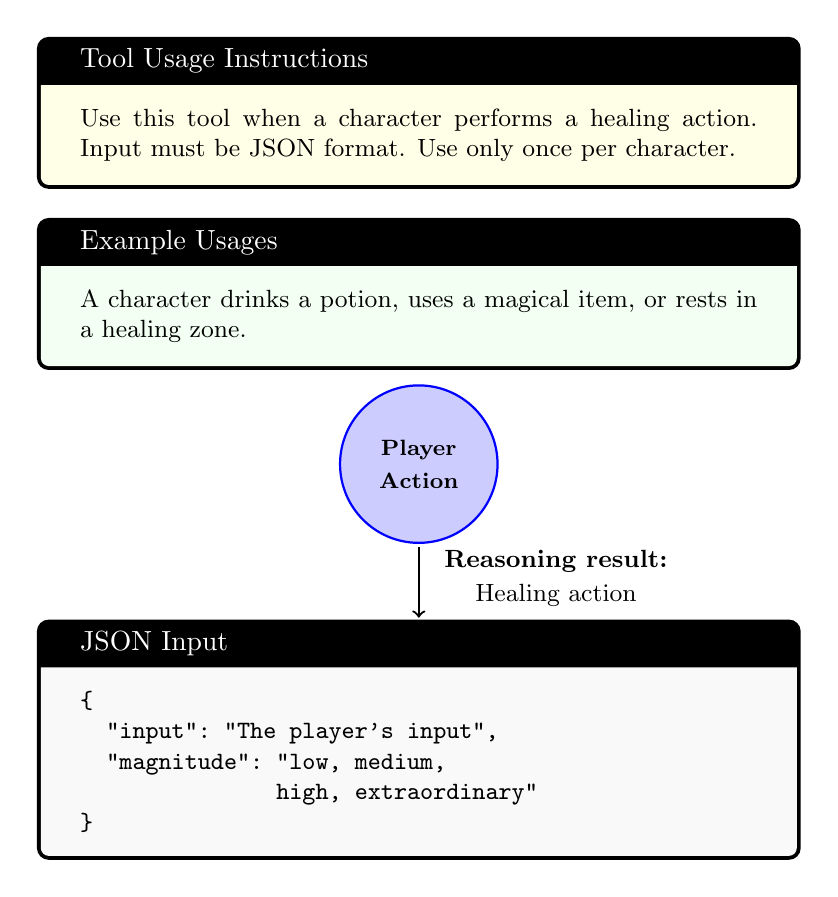
\begin{tikzpicture}
        % Healing action circle
        \draw[fill=blue!20, draw=blue, thick] (0, -1.65) circle (1.0cm);
        \node[text width=1.5cm, align=center] at (0, -1.65) {\footnotesize\textbf{Player Action}};

        % Arrow pointing down
        \draw[->, thick] (0, -2.7) -- (0, -3.6);
        \node[anchor=west, align=center] at (0.2, -3.1) {\small \textbf{Reasoning result:}\\ \small Healing action};

        % JSON Input Box below
        \node[anchor=north] at (0, -3.5) {
 %           \begin{adjustbox}{width=0.3\columnwidth}
            \begin{tcolorbox}[colback=gray!5, colframe=black, title=JSON Input, width=0.8\columnwidth, fontupper=\small]
\begin{verbatim}
{
  "input": "The player's input",
  "magnitude": "low, medium, 
               high, extraordinary"
}
\end{verbatim}
            \end{tcolorbox}
%            \end{adjustbox}
        };

        % Instructions box above
        \node[anchor=north] at (0, 3.9) {
 %           \begin{adjustbox}{width=0.3\columnwidth}
            \begin{tcolorbox}[colback=yellow!10, colframe=black, title=Tool Usage Instructions, width=0.8\columnwidth, fontupper=\small]
            Use this tool when a character performs a healing action. Input must be JSON format. 
            Use only once per character.
            \end{tcolorbox}
%            \end{adjustbox}
        };

        % Example actions box below JSON
        \node[anchor=north] at (0, 1.6) {
 %           \begin{adjustbox}{width=0.3\columnwidth}
            \begin{tcolorbox}[colback=green!5, colframe=black, title=Example Usages
            , width=0.8\columnwidth, fontupper=\small]
            A character drinks a potion, uses a magical item, or rests in a healing zone.
            \end{tcolorbox}
 %           \end{adjustbox}
        };
    \end{tikzpicture}
    \caption{Illustration of the Narrator's reasoning process of using the HealCharacter tool.}
    \Description{An illustration of the Narrator's reasoning process using the HealCharacter tool. Specifically how it is used to determine if a character performs an action that should heal them.}
    \label{fig:healing-tool}
\end{figure}

As agents utilize tool descriptions to guide their reasoning process, all descriptions follow a standardized pattern to ensure consistent behavior:

\begin{enumerate}
    \item \textbf{When to Use:} This step ensures the tool is invoked only under appropriate circumstances, forming the basis of the \textit{Tool Usage Instructions} component of the reasoning process.
    \item \textbf{Examples of Usage:} This step provides sample scenarios for tool application, directly corresponding to the \textit{Example Usages} component. It enables the Narrator agent to associate specific actions with the respective tool.
    \item \textbf{Input Format:} This step defines the input format, which is crucial for accurate parsing by the tools. All input formats are specified in JSON to support consistent interpretation.
    \item \textbf{Number of Uses in Each Trajectory:} This step determines the permissible frequency of tool use within each ReAct trajectory, which corresponds to a single message from the player. It is vital for ensuring agents adhere to the intended usage limits, incorporated into the \textit{Tool Usage Instructions} component.
\end{enumerate}

By adhering to this structured format, the agents are equipped to make informed, consistent decisions, ensuring the execution of tools within the AI GM framework.


%Benefits of v2 approach compared to v1
%\subsection{Design Innovations}

%ChatRPG v2 introduces a dual-agent system—Narrator and Archivist—that leverages the ReAct framework and memory to simulate human-like GM decision-making. The Narrator dynamically adapts the storyline to player interactions, while the Archivist ensures narrative continuity by managing key game elements. This modular design not only enables richer, emergent gameplay and more natural NPC interactions but also simplifies feature integration. Unlike v1’s monolithic approach, v2 supports seamless upgrades by adding new tools without disrupting existing functionality.

\section{Evaluation}

\subsection{Experimental Setup}\label{subsec:exp_setup}

In our evaluation, we adopt \textit{Code-Llama-7B} as the pre-trained model for fine-tuning, employing the low-rank-adaption (QLoRA)~\cite{hu2021lora, dettmers2024qlora} technique for faster training and lower memory consumption. 
Key configurations include loading the model in 8-bit, a sequence length of 4096, sample packing, and padding to sequence length. We set the warmup steps to 100, with a gradient accumulation of 4 steps, a micro-batch size of 4, and an inference batch size of 2.
For both syntax and functionality checks, we measure pass@3 accuracy as metrics. In the ablation study from~\secref{subsec:exp_finetune} to~\secref{subsec:complexity}, we adopt \textit{MachineGen} for evaluation.

Experiments are conducted on a server with four NVIDIA L20 GPUs (48 GB each), an 80 vCPU Intel® Xeon® Platinum 8457C, and 100GB of RAM. This setup ensures sufficient computational power and memory to handle the intensive demands of fine-tuning and inference efficiently, especially for long data sequences in the feedback loop experiment. 

\subsection{Effect of Supervised Finetuning}\label{subsec:exp_finetune}
Our first ablation study investigates the effect of the model fine-tuning.
We evaluated the performance based on both syntax and functionality checks. 
As shown in~\figref{fig:finetune_cot}(a), the results demonstrate that the finetuning dramatically increases syntax correctness from $54.85$\% to $88.44$\%. 
More importantly, the impact of finetuning is even more pronounced in the functionality evaluation, where the non-finetuned model failed to achieve any correct functionality test, but the accuracy is improved to $53.20$\% in the finetuned model. These enhancements highlight the critical role of finetuning in producing not only syntactically correct but also functionally viable codes, which demonstrates the benefits of finetuning LLMs for hardware design in the HLS code generation task.




\subsection{Effect of Chain-of-Thought Prompting}\label{subsec:exp_cot}
To assess the effect of the chain-of-thought (CoT) technique,
we perform both syntax and functionality evaluation on the fine-tuned model with and without the use of CoT.
As indicated in~\figref{fig:finetune_cot}(b), incorporating CoT leads to a noticeable improvement in both metrics. 
Specifically, syntax correctness increases from $88.44$\% to $94.33$\%, and functionality score rises from $53.20$\% to $61.45$\%. 
The result demonstrates the effectiveness of CoT in enhancing the reasoning capability, thereby improving its overall performance.


\subsection{Effect of Feedback Loops}\label{subsec:exp_feedback}
Our two-step feedback loop provides both syntax and functionality feedback. We evaluate the impact of these feedback loops with different numbers of iterations, ranging from 0 to 2.The results, shown in Figure ~\figref{fig:syntax_feedback} and ~\figref{fig:func_feedback}, indicate that both syntax and functionality feedback loops significantly improve model performance, especially when combined with COT prompting. The initial feedback loop yields substantial accuracy improvements in both syntax correctness and functionality evaluation, though the second loop shows diminishing returns.Syntax feedback loops enhance both syntax correctness and functionality performance, suggesting that iterative refinement is particularly effective for complex tasks. Similarly, functionality feedback loops not only improve functionality checks but also boost syntax accuracy, indicating that enhancements in functional understanding contribute to better syntactic performance.

 \begin{figure}[t]
    \centering
    \includegraphics[width=1\linewidth]{./figures/merged_finetune_cot.pdf}
    \vspace{-5mm}
    \caption{Effect of fine-tuning and chain-of-thought.}
    \label{fig:finetune_cot}
\end{figure}

\begin{figure}[t]
    \centering
    \includegraphics[width=0.95\linewidth]{./figures/Effect_of_Syntax_Feedback_Loop.pdf}
    \vspace{-2mm}
    \caption{Effect of syntax feedback loop.}
    \vspace{-2mm}
    \label{fig:syntax_feedback}
\end{figure}
\begin{figure}[t]
    \centering
    \includegraphics[width=0.95\linewidth]{./figures/Effect_of_Functionality_Feedback_Loop.pdf}
    \caption{Effect of functionality feedback loop.}
    \vspace{-2mm}
    \label{fig:func_feedback}
\end{figure}


\subsection{Time Cost and Hardware Performance}\label{subsec:exp_timecost}

\figref{fig:time_cost} shows the time cost for generating 120 data entries under different conditions, measuring the impact of CoT and feedback loops. Without a feedback loop, CoT significantly reduces the time. Adding a syntax feedback loop increases the time, but CoT continues to notably decrease the duration. The functionality feedback loop is the most time-consuming, though CoT still provides a notable reduction, albeit less dramatic. This demonstrates CoT's effectiveness in reducing operational times across varying complexities.

For the test set,
we evaluate the latency and resource consumption of the generated \textit{HLS} designs using a Xilinx VCU118 as our target FPGA, with a clock frequency of $200$MHz and Xilinx Vivado 2020.1 for synthesis.
As shown in~\tabref{tb:perf_resource}, all \textit{HLS} designs demonstrate reasonable performance, with BRAM usage consistently remained at zero due to the design scale.

\begin{figure}
    \centering
    \includegraphics[width=0.95\linewidth]{./figures/Time_Cost_Analysis.pdf}
    \vspace{-2mm}
    \caption{Time cost of code generation.}
    \label{fig:time_cost}
\end{figure}


\begin{table}[htb]
\centering
\caption{Latency and resource usage of LLM-generated designs synthesized on a VCU118 FPGA.}
\label{tb:perf_resource}
\setlength\tabcolsep{1pt} 
\scalebox{0.8}{
% \begin{tabular}{L{2cm}ccC{1.5cm}C{2.5cm}}
\begin{tabular}{C{2.5cm}|C{1.9cm}|C{1.5cm}|C{1.5cm}|C{1.3cm}|C{1.3cm}}
\toprule
{}& \textbf{Latency} (ms)& \textbf{LUTs} & \textbf{Registers} & \textbf{DSP48s} & \textbf{BRAMs} \\ \midrule
{\textbf{Available}} & - & 1182240 & 2364480 & 6840 & 4320 \\ \midrule
{\textit{ellpack}} & 0.304 & 1011 & 1079 & 11 & 0 \\
{\textit{syrk}} & 21.537 & 1371 & 1621 & 19 & 0 \\
{\textit{syr2k}} & 40.626 & 1572 & 1771 & 19 & 0 \\
{\textit{stencil2d}} & 1.368 & 287 & 123 & 3 & 0 \\
{\textit{trmm-opt}} & 15.889 & 1262 & 1239 & 11 & 0 \\
{\textit{stencil3d}} & 21.537 & 1173 & 1271 & 20 & 0 \\
{\textit{symm}} & 24.601 & 1495 & 1777 & 19 & 0 \\
{\textit{symm-opt}} & 16.153 & 1361 & 1608 & 19 & 0 \\
{\textit{symm-opt-medium}} & 579.0 & 2223 & 2245 & 22 & 0 \\
\bottomrule
\end{tabular}}
\end{table}

\subsection{Effect of Task Complexity}\label{subsec:complexity}
We analyze the effects of code complexity on the performance of fine-tuning our language model with CoT prompting and tested without the use of any feedback loops during inference. 
We categorize \textit{MachineGen} into three classes according to their code complexity: easy, medium, and difficult.
The results shown in the \tabref{tab:model_performance} indicates a clear trend: as the complexity of the generated code increases, both syntax and functionality correctness rates decline. This outcome could be attributed to several factors. First, more complex code inherently presents more challenges in maintaining syntactic integrity and functional accuracy. Second, the absence of feedback loops in the inference phase may have limited the model's ability to self-correct emerging errors in more complicated code generations.

\begin{table}[h]
\centering
\caption{Performance across different complexity levels.}
\scalebox{0.8}{
\begin{tabular}{c|c|c}
\hline
\textbf{Test Set} & \textbf{Syntax Check} & \textbf{Functionality} \\
\hline
Easy & 96.67\% & 63.33\% \\
Medium & 96.67\% & 53.33\% \\
Difficult & 90\% & 53.33\% \\
\hline
\end{tabular}}
\label{tab:model_performance}
\end{table}

\subsection{Analysis of \textit{MachineGen} and \textit{HumanRefine}}
\begin{table}[h]
\centering
\caption{Performance on \textit{MachineGen} and \textit{HumanRefine}.}
\scalebox{0.9}{
\begin{tabular}{c|c|c}
\hline
\textbf{Test Set} & \textbf{Syntax Check} & \textbf{Functionality Check} \\
\hline
\textit{MachineGen} & 93.83\% & 62.24\% \\
\hline
\textit{HumanRefine} & 47.29\% & 21.36\% \\
\hline
\end{tabular}}
\vspace{-3mm}
\label{table:eval_comparison}
\end{table}

As shown in~\tabref{table:eval_comparison}, this section compares the performance of our model on \textit{MachineGen} and \textit{HumanRefine} test sets.
Our findings reveal that the performance on the \textit{HumanRefine} is significantly lower than on the \textit{MachineGen}. This disparity suggests that the model is more adept at handling machine-generated prompts. The primary reasons for this are: the model's training data bias towards machine-generated prompts, the increased complexity and nuanced nature of human-generated prompts, and the conciseness and clarity of human-generated prompts that often omit repetitive or explicit details found in machine-generated prompts, making it harder for the model to generate syntactically and functionally correct code.

\subsection{Thoughts, Insights, and Limitations}

\noindent \textbf{1. \textit{HLS} versus \textit{HDL} for AI-assisted code generation:} The selection of programming language for hardware code generation should mainly depend on two  factors:
\begin{itemize}[leftmargin=*]
    \item \textit{Quality of Generated Hardware Design}: The evaluation of hardware design's quality includes syntax correctness, functionality, and hardware performance.
    Since \textit{HLS} shares similar semantics and syntax with programming languages commonly used during LLM pre-training, this work demonstrates that the LLM-assisted code generation for \textit{HLS} has the potential to achieve high syntax and functional correctness in hardware designs. While this work does not leverage hardware performance as feedback for design generation, it identifies this aspect as a key direction for future research and enhancements.
    \item \textit{Runtime Cost of Hardware Generation}: Although \textit{HLS}-based designs typically require fewer tokens compared to \textit{HDL} during the code generation phase—suggesting potentially lower costs—the overall runtime costs associated with HLS synthesis must also be considered. A more comprehensive quantitative comparison of these runtime costs is planned for our future work. 
\end{itemize}

\noindent \textbf{2. Input instructions and datasets are crucial}: The fine-tuning of pre-trained LLMs on \textit{HLS} dataset can bring a significant improvement in the design quality, echoing findings from previous studies on \textit{Verilog} code generation~\cite{thakur2023verigen}. 
Additionally, during our evaluation, we found that employing simple CoT prompting largely improves hardware design quality. 
This result contrasts with the application of CoT in general-purpose programming languages, where a specialized form of CoT is necessary~\cite{li2023structured}.
Therefore, future efforts for further enhancement can focus on collecting high-quality datasets and exploring better refinement of input prompts.

\noindent \textbf{3. Limitations}: At the time of this research, more advanced reasoning models, such as DeepSeek-R1~\cite{guo2025deepseek}, were not available for evaluation. Additionally, test-time scaling approaches~\cite{welleck2024decoding} could be incorporated to further enhance performance in the future.
Moreover, we observe that the diversity of hardware designs in the benchmark is limited, which may impact the generalizability of our findings.
We intend to address these limitations in our future work.


%% New Disucssion 
Our study reveals how heavy users integrate LLMs into their daily tasks through distinct patterns. Rather than simple tool usage, participants demonstrated sophisticated cognitive offloading strategies that transformed their decision-making processes. In our study, we observed participants delegating social and interpersonal reasoning to LLMs, suggesting ways users might leverage AI collaboration to support their social cognition processes.

Participants' mental models of LLMs directly influenced their cognitive strategies---those viewing LLMs as rational entities engaged in cognitive complementarity by leveraging LLM capabilities where they perceived personal limitations, while those viewing LLMs as average decision-makers used cognitive benchmarking, establishing baseline standards while reserving higher-order tasks for themselves.
% While delegating a broad range of decisions raised potential concerns about over-reliance and diminished critical thinking, our findings also highlight a nuanced form of human-AI collaboration where users and LLMs develop complementary relationships. Participants showed diverse usage strategies, treating LLMs as an emerging problem-solving tool and developing sophisticated prompting techniques. Most notably, participants frequently sought LLM guidance on social appropriateness and interpersonal situations. Although some users expressed concerns about potential skill degradation and a sense of unease, LLM consultations often led to a more thorough consideration of social factors and an enhanced understanding of different perspectives.

This raises questions for future research on redefining how we conceptualize and measure over-reliance on LLMs. Current metrics typically assess over-reliance through simplified quantitative measures in controlled settings, primarily focusing on users' acceptance rates of LLM outputs ~\cite{bo2024rely, kim2024rely}. However, our findings reveal more complex patterns of engagement. Participants did not blindly adopt LLM outputs, even in cases where they eventually accepted them. Instead, participants demonstrated thoughtful delegation strategies, using LLMs to validate existing decisions, automate routine tasks, or navigate unfamiliar situations. The critical concern was not users' acceptance of LLM outputs, but rather instances where users adopted LLM reasoning without exploring alternative perspectives. Future research should expand the definition of over-reliance beyond simple acceptance rates to examine how users critically engage with alternative lines of reasoning.

Another key direction for future research involves capturing diverse user contexts. Our participants valued the ability of LLMs to extract necessary contextual information when not initially provided. They appreciated that they could receive meaningful responses without extensively explaining background information, even for context-heavy topics like relationship advice. Future research should explore ways to incorporate multi-modal inputs beyond text-based interactions, allowing users to convey context through various channels. Additionally, LLMs' ability to elicit implicit user intentions without explicit prompting is crucial, as demonstrated by recent advances in reasoning-focused LLM architectures that can proactively identify and address underlying user needs.

The development of active usage patterns with LLMs appeared more prominent among younger users who had less experience managing tasks without these systems. Participants with extensive pre-LLM experience maintained clearer boundaries and showed greater awareness of system limitations. In contrast, users with less experience with LLMs demonstrated fewer reservations, viewing LLM interaction itself as a skill and actively developing their prompting strategies. Conducting design studies focused on younger generations, to better understand and support these emerging interaction patterns represents a crucial direction for future research.

\section{Discussion}\label{sec:discussion}



\subsection{From Interactive Prompting to Interactive Multi-modal Prompting}
The rapid advancements of large pre-trained generative models including large language models and text-to-image generation models, have inspired many HCI researchers to develop interactive tools to support users in crafting appropriate prompts.
% Studies on this topic in last two years' HCI conferences are predominantly focused on helping users refine single-modality textual prompts.
Many previous studies are focused on helping users refine single-modality textual prompts.
However, for many real-world applications concerning data beyond text modality, such as multi-modal AI and embodied intelligence, information from other modalities is essential in constructing sophisticated multi-modal prompts that fully convey users' instruction.
This demand inspires some researchers to develop multimodal prompting interactions to facilitate generation tasks ranging from visual modality image generation~\cite{wang2024promptcharm, promptpaint} to textual modality story generation~\cite{chung2022tale}.
% Some previous studies contributed relevant findings on this topic. 
Specifically, for the image generation task, recent studies have contributed some relevant findings on multi-modal prompting.
For example, PromptCharm~\cite{wang2024promptcharm} discovers the importance of multimodal feedback in refining initial text-based prompting in diffusion models.
However, the multi-modal interactions in PromptCharm are mainly focused on the feedback empowered the inpainting function, instead of supporting initial multimodal sketch-prompt control. 

\begin{figure*}[t]
    \centering
    \includegraphics[width=0.9\textwidth]{src/img/novice_expert.pdf}
    \vspace{-2mm}
    \caption{The comparison between novice and expert participants in painting reveals that experts produce more accurate and fine-grained sketches, resulting in closer alignment with reference images in close-ended tasks. Conversely, in open-ended tasks, expert fine-grained strokes fail to generate precise results due to \tool's lack of control at the thin stroke level.}
    \Description{The comparison between novice and expert participants in painting reveals that experts produce more accurate and fine-grained sketches, resulting in closer alignment with reference images in close-ended tasks. Novice users create rougher sketches with less accuracy in shape. Conversely, in open-ended tasks, expert fine-grained strokes fail to generate precise results due to \tool's lack of control at the thin stroke level, while novice users' broader strokes yield results more aligned with their sketches.}
    \label{fig:novice_expert}
    % \vspace{-3mm}
\end{figure*}


% In particular, in the initial control input, users are unable to explicitly specify multi-modal generation intents.
In another example, PromptPaint~\cite{promptpaint} stresses the importance of paint-medium-like interactions and introduces Prompt stencil functions that allow users to perform fine-grained controls with localized image generation. 
However, insufficient spatial control (\eg, PromptPaint only allows for single-object prompt stencil at a time) and unstable models can still leave some users feeling the uncertainty of AI and a varying degree of ownership of the generated artwork~\cite{promptpaint}.
% As a result, the gap between intuitive multi-modal or paint-medium-like control and the current prompting interface still exists, which requires further research on multi-modal prompting interactions.
From this perspective, our work seeks to further enhance multi-object spatial-semantic prompting control by users' natural sketching.
However, there are still some challenges to be resolved, such as consistent multi-object generation in multiple rounds to increase stability and improved understanding of user sketches.   


% \new{
% From this perspective, our work is a step forward in this direction by allowing multi-object spatial-semantic prompting control by users' natural sketching, which considers the interplay between multiple sketch regions.
% % To further advance the multi-modal prompting experience, there are some aspects we identify to be important.
% % One of the important aspects is enhancing the consistency and stability of multiple rounds of generation to reduce the uncertainty and loss of control on users' part.
% % For this purpose, we need to develop techniques to incorporate consistent generation~\cite{tewel2024training} into multi-modal prompting framework.}
% % Another important aspect is improving generative models' understanding of the implicit user intents \new{implied by the paint-medium-like or sketch-based input (\eg, sketch of two people with their hands slightly overlapping indicates holding hand without needing explicit prompt).
% % This can facilitate more natural control and alleviate users' effort in tuning the textual prompt.
% % In addition, it can increase users' sense of ownership as the generated results can be more aligned with their sketching intents.
% }
% For example, when users draw sketches of two people with their hands slightly overlapping, current region-based models cannot automatically infer users' implicit intention that the two people are holding hands.
% Instead, they still require users to explicitly specify in the prompt such relationship.
% \tool addresses this through sketch-aware prompt recommendation to fill in the necessary semantic information, alleviating users' workload.
% However, some users want the generative AI in the future to be able to directly infer this natural implicit intentions from the sketches without additional prompting since prompt recommendation can still be unstable sometimes.


% \new{
% Besides visual generation, 
% }
% For example, one of the important aspect is referring~\cite{he2024multi}, linking specific text semantics with specific spatial object, which is partly what we do in our sketch-aware prompt recommendation.
% Analogously, in natural communication between humans, text or audio alone often cannot suffice in expressing the speakers' intentions, and speakers often need to refer to an existing spatial object or draw out an illustration of her ideas for better explanation.
% Philosophically, we HCI researchers are mostly concerned about the human-end experience in human-AI communications.
% However, studies on prompting is unique in that we should not just care about the human-end interaction, but also make sure that AI can really get what the human means and produce intention-aligned output.
% Such consideration can drastically impact the design of prompting interactions in human-AI collaboration applications.
% On this note, although studies on multi-modal interactions is a well-established topic in HCI community, it remains a challenging problem what kind of multi-modal information is really effective in helping humans convey their ideas to current and next generation large AI models.




\subsection{Novice Performance vs. Expert Performance}\label{sec:nVe}
In this section we discuss the performance difference between novice and expert regarding experience in painting and prompting.
First, regarding painting skills, some participants with experience (4/12) preferred to draw accurate and fine-grained shapes at the beginning. 
All novice users (5/12) draw rough and less accurate shapes, while some participants with basic painting skills (3/12) also favored sketching rough areas of objects, as exemplified in Figure~\ref{fig:novice_expert}.
The experienced participants using fine-grained strokes (4/12, none of whom were experienced in prompting) achieved higher IoU scores (0.557) in the close-ended task (0.535) when using \tool. 
This is because their sketches were closer in shape and location to the reference, making the single object decomposition result more accurate.
Also, experienced participants are better at arranging spatial location and size of objects than novice participants.
However, some experienced participants (3/12) have mentioned that the fine-grained stroke sometimes makes them frustrated.
As P1's comment for his result in open-ended task: "\emph{It seems it cannot understand thin strokes; even if the shape is accurate, it can only generate content roughly around the area, especially when there is overlapping.}" 
This suggests that while \tool\ provides rough control to produce reasonably fine results from less accurate sketches for novice users, it may disappoint experienced users seeking more precise control through finer strokes. 
As shown in the last column in Figure~\ref{fig:novice_expert}, the dragon hovering in the sky was wrongly turned into a standing large dragon by \tool.

Second, regarding prompting skills, 3 out of 12 participants had one or more years of experience in T2I prompting. These participants used more modifiers than others during both T2I and R2I tasks.
Their performance in the T2I (0.335) and R2I (0.469) tasks showed higher scores than the average T2I (0.314) and R2I (0.418), but there was no performance improvement with \tool\ between their results (0.508) and the overall average score (0.528). 
This indicates that \tool\ can assist novice users in prompting, enabling them to produce satisfactory images similar to those created by users with prompting expertise.



\subsection{Applicability of \tool}
The feedback from user study highlighted several potential applications for our system. 
Three participants (P2, P6, P8) mentioned its possible use in commercial advertising design, emphasizing the importance of controllability for such work. 
They noted that the system's flexibility allows designers to quickly experiment with different settings.
Some participants (N = 3) also mentioned its potential for digital asset creation, particularly for game asset design. 
P7, a game mod developer, found the system highly useful for mod development. 
He explained: "\emph{Mods often require a series of images with a consistent theme and specific spatial requirements. 
For example, in a sacrifice scene, how the objects are arranged is closely tied to the mod's background. It would be difficult for a developer without professional skills, but with this system, it is possible to quickly construct such images}."
A few participants expressed similar thoughts regarding its use in scene construction, such as in film production. 
An interesting suggestion came from participant P4, who proposed its application in crime scene description. 
She pointed out that witnesses are often not skilled artists, and typically describe crime scenes verbally while someone else illustrates their account. 
With this system, witnesses could more easily express what they saw themselves, potentially producing depictions closer to the real events. "\emph{Details like object locations and distances from buildings can be easily conveyed using the system}," she added.

% \subsection{Model Understanding of Users' Implicit Intents}
% In region-sketch-based control of generative models, a significant gap between interaction design and actual implementation is the model's failure in understanding users' naturally expressed intentions.
% For example, when users draw sketches of two people with their hands slightly overlapping, current region-based models cannot automatically infer users' implicit intention that the two people are holding hands.
% Instead, they still require users to explicitly specify in the prompt such relationship.
% \tool addresses this through sketch-aware prompt recommendation to fill in the necessary semantic information, alleviating users' workload.
% However, some users want the generative AI in the future to be able to directly infer this natural implicit intentions from the sketches without additional prompting since prompt recommendation can still be unstable sometimes.
% This problem reflects a more general dilemma, which ubiquitously exists in all forms of conditioned control for generative models such as canny or scribble control.
% This is because all the control models are trained on pairs of explicit control signal and target image, which is lacking further interpretation or customization of the user intentions behind the seemingly straightforward input.
% For another example, the generative models cannot understand what abstraction level the user has in mind for her personal scribbles.
% Such problems leave more challenges to be addressed by future human-AI co-creation research.
% One possible direction is fine-tuning the conditioned models on individual user's conditioned control data to provide more customized interpretation. 

% \subsection{Balance between recommendation and autonomy}
% AIGC tools are a typical example of 
\subsection{Progressive Sketching}
Currently \tool is mainly aimed at novice users who are only capable of creating very rough sketches by themselves.
However, more accomplished painters or even professional artists typically have a coarse-to-fine creative process. 
Such a process is most evident in painting styles like traditional oil painting or digital impasto painting, where artists first quickly lay down large color patches to outline the most primitive proportion and structure of visual elements.
After that, the artists will progressively add layers of finer color strokes to the canvas to gradually refine the painting to an exquisite piece of artwork.
One participant in our user study (P1) , as a professional painter, has mentioned a similar point "\emph{
I think it is useful for laying out the big picture, give some inspirations for the initial drawing stage}."
Therefore, rough sketch also plays a part in the professional artists' creation process, yet it is more challenging to integrate AI into this more complex coarse-to-fine procedure.
Particularly, artists would like to preserve some of their finer strokes in later progression, not just the shape of the initial sketch.
In addition, instead of requiring the tool to generate a finished piece of artwork, some artists may prefer a model that can generate another more accurate sketch based on the initial one, and leave the final coloring and refining to the artists themselves.
To accommodate these diverse progressive sketching requirements, a more advanced sketch-based AI-assisted creation tool should be developed that can seamlessly enable artist intervention at any stage of the sketch and maximally preserve their creative intents to the finest level. 

\subsection{Ethical Issues}
Intellectual property and unethical misuse are two potential ethical concerns of AI-assisted creative tools, particularly those targeting novice users.
In terms of intellectual property, \tool hands over to novice users more control, giving them a higher sense of ownership of the creation.
However, the question still remains: how much contribution from the user's part constitutes full authorship of the artwork?
As \tool still relies on backbone generative models which may be trained on uncopyrighted data largely responsible for turning the sketch into finished artwork, we should design some mechanisms to circumvent this risk.
For example, we can allow artists to upload backbone models trained on their own artworks to integrate with our sketch control.
Regarding unethical misuse, \tool makes fine-grained spatial control more accessible to novice users, who may maliciously generate inappropriate content such as more realistic deepfake with specific postures they want or other explicit content.
To address this issue, we plan to incorporate a more sophisticated filtering mechanism that can detect and screen unethical content with more complex spatial-semantic conditions. 
% In the future, we plan to enable artists to upload their own style model

% \subsection{From interactive prompting to interactive spatial prompting}


\subsection{Limitations and Future work}

    \textbf{User Study Design}. Our open-ended task assesses the usability of \tool's system features in general use cases. To further examine aspects such as creativity and controllability across different methods, the open-ended task could be improved by incorporating baselines to provide more insightful comparative analysis. 
    Besides, in close-ended tasks, while the fixing order of tool usage prevents prior knowledge leakage, it might introduce learning effects. In our study, we include practice sessions for the three systems before the formal task to mitigate these effects. In the future, utilizing parallel tests (\textit{e.g.} different content with the same difficulty) or adding a control group could further reduce the learning effects.

    \textbf{Failure Cases}. There are certain failure cases with \tool that can limit its usability. 
    Firstly, when there are three or more objects with similar semantics, objects may still be missing despite prompt recommendations. 
    Secondly, if an object's stroke is thin, \tool may incorrectly interpret it as a full area, as demonstrated in the expert results of the open-ended task in Figure~\ref{fig:novice_expert}. 
    Finally, sometimes inclusion relationships (\textit{e.g.} inside) between objects cannot be generated correctly, partially due to biases in the base model that lack training samples with such relationship. 

    \textbf{More support for single object adjustment}.
    Participants (N=4) suggested that additional control features should be introduced, beyond just adjusting size and location. They noted that when objects overlap, they cannot freely control which object appears on top or which should be covered, and overlapping areas are currently not allowed.
    They proposed adding features such as layer control and depth control within the single-object mask manipulation. Currently, the system assigns layers based on color order, but future versions should allow users to adjust the layer of each object freely, while considering weighted prompts for overlapping areas.

    \textbf{More customized generation ability}.
    Our current system is built around a single model $ColorfulXL-Lightning$, which limits its ability to fully support the diverse creative needs of users. Feedback from participants has indicated a strong desire for more flexibility in style and personalization, such as integrating fine-tuned models that cater to specific artistic styles or individual preferences. 
    This limitation restricts the ability to adapt to varied creative intents across different users and contexts.
    In future iterations, we plan to address this by embedding a model selection feature, allowing users to choose from a variety of pre-trained or custom fine-tuned models that better align with their stylistic preferences. 
    
    \textbf{Integrate other model functions}.
    Our current system is compatible with many existing tools, such as Promptist~\cite{hao2024optimizing} and Magic Prompt, allowing users to iteratively generate prompts for single objects. However, the integration of these functions is somewhat limited in scope, and users may benefit from a broader range of interactive options, especially for more complex generation tasks. Additionally, for multimodal large models, users can currently explore using affordable or open-source models like Qwen2-VL~\cite{qwen} and InternVL2-Llama3~\cite{llama}, which have demonstrated solid inference performance in our tests. While GPT-4o remains a leading choice, alternative models also offer competitive results.
    Moving forward, we aim to integrate more multimodal large models into the system, giving users the flexibility to choose the models that best fit their needs. 
    


\section{Conclusion}\label{sec:conclusion}
In this paper, we present \tool, an interactive system designed to help novice users create high-quality, fine-grained images that align with their intentions based on rough sketches. 
The system first refines the user's initial prompt into a complete and coherent one that matches the rough sketch, ensuring the generated results are both stable, coherent and high quality.
To further support users in achieving fine-grained alignment between the generated image and their creative intent without requiring professional skills, we introduce a decompose-and-recompose strategy. 
This allows users to select desired, refined object shapes for individual decomposed objects and then recombine them, providing flexible mask manipulation for precise spatial control.
The framework operates through a coarse-to-fine process, enabling iterative and fine-grained control that is not possible with traditional end-to-end generation methods. 
Our user study demonstrates that \tool offers novice users enhanced flexibility in control and fine-grained alignment between their intentions and the generated images.



%%
%% The acknowledgments section is defined using the "acks" environment
%% (and NOT an unnumbered section). This ensures the proper
%% identification of the section in the article metadata, and the
%% consistent spelling of the heading.

\begin{acks}
We sincerely thank the 12 test participants whose contributions through user tests were essential in shaping the outcomes of this study.
\end{acks}

%%
%% The next two lines define the bibliography style to be used, and
%% the bibliography file.
\bibliographystyle{ACM-Reference-Format}
\balance
\bibliography{references}


%%
%% If your work has an appendix, this is the place to put it.
\appendix



\begingroup
\onecolumn
\parindent0pt

\section{Appendix Overview} \label{app_overview}

The following sections provide the text used in the prompts for ChatRPG v1 and the narrator and archivist agents in the game master AI system v2. These files will be shared on the project's Github repository to enable others to reuse the system and adapt it to their needs. 

In addition, the questions used in the comparative evaluation are provided. These questions were used to measure the participant's experience with ChatRPG. The survey is based partly on the Player Experience Inventory (PXI) with additional questions focused on the RPG experience.

\section{ChatRPG v1 Prompts} \label{app_chatgpt_v1_prompts}

\textbf{Initial Game-Start Prompt}
You are an expert game master in an RPG. You direct the narrative and control non-player characters. The player's adventure has just begun. You must provide an in-depth introduction to the campaign. Address the player in the second person. Always respond in valid JSON, and in this exact structure: \{ "narrative": "", "characters": [ ], "environment": \{\}, "opponent": "name of current opponent, if any" \} Where "characters" includes any new characters met by the player, describing them concisely here in this way: \{ "name": "Name of the character", "description": "Short description", "type": "Humanoid, SmallCreature, LargeCreature or Monster" \}. "environment" is filled out when the player enters a new location, describe it shortly here in the format: \{ "name": "environment", "description": "short description" \}.

\textbf{CombatHitHit}
You are an expert game master in a single-player RPG. The player is in combat with an opponent. You will be given information about an attack that the player has done and the damage it will deal. Your job is to provide flavor text regarding this attack, including the damage dealt. The player's attack always hits. You should afterward provide flavor text regarding the opponent's attack towards the player, including the damage dealt. The opponent's attack always hits. The damage of the opponent's attack is also provided. Your response should account for how large of a ratio the damage dealt is compared to the opponent's current health points. For example, if the opponent's current health points are high, they will not be heavily wounded by low damage. You should also account for the ratio of current health points to maximum health points for both the player and the opponent when describing their behavior. Address the player in the second person. Always respond in valid JSON, and in this exact structure: \{ "narrative": "", "characters": [ ], "environment": \{\}, "opponent": "name of current opponent, if any" \}.

\textbf{CombatHitMiss}
You are an expert game master in a single-player RPG. The player is in combat with an opponent. You will be given information about an attack that the player has done and the damage it will deal. Your job is to provide flavor text regarding this attack, including the damage dealt. The player's attack always hits. You should afterward provide flavor text regarding the opponent's attack towards the player. The opponent's attack will miss. For both flavor texts, you may utilize the information in the provided conversation. Your response should account for how large of a ratio the damage dealt is compared to the opponent's current health points. For example, if the opponent's current health points are high, they will not be heavily wounded by low damage. You should also account for the ratio of current health points to maximum health points for both the player and the opponent when describing their behavior. Address the player in the second person. Always respond in valid JSON, and in this exact structure: \{ "narrative": "", "characters": [ ], "environment": \{\}, "opponent": "name of current opponent" \}.

\textbf{CombatMissHit}
You are an expert game master in a single-player RPG. The player is in combat with an opponent. You will be given information about an attack that the player has done. Your job is to provide flavor text regarding this attack. The player's attack always misses. You should afterward provide flavor text regarding the opponent's attack towards the player, including the damage dealt. The opponent's attack always hits. The damage of the opponent's attack is also provided. For both flavor texts, you may utilize the information in the provided conversation. Your response should account for how large of a ratio the damage dealt is compared to the opponent's current health points. For example, if the opponent's current health points are high, they will not be heavily wounded by low damage. You should also account for the ratio of current health points to maximum health points for both the player and the opponent when describing their behavior. Address the player in the second person. Always respond in valid JSON, and in this exact structure: \{ "narrative": "", "characters": [ ], "environment": \{\}, "opponent": "name of current opponent" \}.

\textbf{CombatMissMiss}
You are an expert game master in a single-player RPG. The player is in combat with an opponent. You will be given information about an attack that the player has done. Your job is to provide flavor text regarding this attack. The player's attack always misses. You should afterward provide flavor text regarding the opponent's attack towards the player. The opponent's attack always misses. For both flavor texts, you may utilize the information in the provided conversation. Your response should account for how large of a ratio the damage dealt is compared to the opponent's current health points. For example, if the opponent's current health points are high, they will not be heavily wounded by low damage. You should also account for the ratio of current health points to maximum health points for both the player and the opponent when describing their behavior. Address the player in the second person. Always respond in valid JSON, and in this exact structure: \{ "narrative": "", "characters": [ ], "environment": \{\}, "opponent": "name of current opponent" \}.

\textbf{CombatOpponentDescription}
You are an expert game master in a single-player RPG. The player is in combat with an opponent. The player has just attacked someone. Your job is to determine who the player is attacking. Always respond in valid JSON, and in this exact structure: \{ "opponent": "name of current opponent", "characters": [ ] \}, where "characters" includes whoever the user is attacking if they have not previously appeared in the narrative, describing them concisely here in this exact way: \{ "name": "Name of the character", "description": "Short description", "type": "Humanoid, SmallCreature, LargeCreature or Monster" \}.

\textbf{DoActionHurtOrHeal}
You are an expert game master in a single-player RPG. The player has just input an action that they want to perform. Your job is to determine whether the player's action will hurt them, heal them, or both. For example, the player could stab themselves, which would hurt them. The player could also drink a potion or take a short rest, which would heal them. Always respond in valid JSON, and in this exact structure: \{ "hurt": true/false, "heal": true/false \}.

\textbf{DoAction}
You are an expert game master in an RPG. You direct the narrative and control non-player characters. The player has input an action that they would like to perform. You must describe everything that happens as the player completes this action. You may have the player say and do anything as long as it is in character. If the player tries to harm someone else, do not explicitly state whether it was successful or not. Address the player in the second person. Always respond in valid JSON, and in this exact structure: \{ "narrative": "", "characters": [ ], "environment": \{\}, "opponent": "name of current opponent, if any" \} Where "characters" includes any new characters met by the player, describing them concisely here in this way: \{ "name": "Name of the character", "description": "Short description", "type": "Humanoid, SmallCreature, LargeCreature or Monster" \}. "environment" is filled out when the player enters a new location, describe it shortly here in the format: \{ "name": "environment", "description": "short description" \}.

\textbf{SayAction}
You are an expert game master in an RPG. You direct the narrative and control non-player characters. The player has input something that they want to say. You must describe how characters react and what they say. Address the player in the second person. Always respond in valid JSON, and in this exact structure: \{ "narrative": "", "characters": [ ], "environment": \{\}, "opponent": "name of current opponent, if any" \} Where "characters" includes any new characters met by the player, describing them concisely here in this way: \{ "name": "Name of the character", "description": "Short description", "type": "Humanoid, SmallCreature, LargeCreature or Monster" \}. "environment" is filled out when the player enters a new location, describe it shortly here in the format: \{ "name": "environment", "description": "short description" \}.



\section{ChatRPG v2 Narrator and Archivist Prompts} \label{app_chatgpt_v2_prompts}

\textbf{Narrator ReAct Prompt}:\\
Assistant is a large language model trained by OpenAI. Assistant is an expert game master in a single-player RPG. Assistant is designed to be able to assist with a wide range of tasks, from directing the narrative and controlling non-player characters. As a language model, Assistant is able to generate human-like text based on the input it receives, allowing it to engage in natural-sounding conversations and provide responses that are coherent and relevant to the topic at hand. Assistant is constantly learning and improving, and its capabilities are constantly evolving. It is able to process and understand large amounts of text, and can use this knowledge to provide an engaging and immersive narrative in response to a wide range of player actions. Additionally, Assistant is able to generate its own text based on the input it receives, allowing it to engage in reasoning about the narrative and provide explanations and descriptions on a wide range of RPG concepts. Overall, Assistant is a powerful tool that can help with a wide range of tasks and provide valuable narratives as an expert game master in a RPG. Assistant must end up with a narrative answer once it has resolved the players actions. Use observations to flesh out the narrative. Make sure to always provide immersive and engaging leads in the narrative. Give the player clues, options for interaction, and make sure to keep the story going forward. Health value numbers must not be mentioned in the narrative, but should inform the descriptions. TOOLS: ------ Assistant has access to the following tools: \{tools\} To use a tool, please use the following format: Thought: Do I need to use a tool? Yes Action: the action to take, should be one of [\{tool\_names\}] Action Input: the input to the action Observation:\textbackslash{}n the result of the action When you have a response to say to the Player, you have resolved the Player's action, or if you do not need to use a tool, you MUST use the format: Thought: Do I need to use a tool? No Final Answer: [your response here] Always add [END] after final answer Begin! Answer length: Concise and only a few, engaging sentences. Game summary: \{summary\} It is important that Assistant take the following into account when constructing the narrative: \{action\} Remember to follow the Thought-Action-Observation format and use Final Answer if you do not need a tool. Always add [END] after final answer. New input: \{input\} Previous tool steps: \{history\}\\

\textbf{Initial Game-Start Prompt}\\
The player's adventure has just begun. You must provide an in-depth introduction to the campaign. Address the player in the second person.\\

\textbf{Do-Action Prompt}\\
The player has input an action that they would like to perform. You must describe everything that happens as the player completes this action. You may have the player say and do anything as long as it is in character. Address the player only in the second person. Always respond in a narrative as the game master in an immersive way.\\

\textbf{Say-Action Prompt}\\
The player has input something that they want to say. You must describe how characters react and what they say. Address the player only in the second person. Always respond in a narrative as the game master in an immersive way.\\

\textbf{Archivist Campaign-Update ReAct Prompt}\\
Assistant is a large language model trained by OpenAI. Assistant is an expert game master in a single-player RPG and a skilled archivist who is able to track changes in a developing world. Assistant is designed to be able to assist with a wide range of tasks, from maintaining the game state and updating the characters and environments in the game. As a language model, Assistant is able to generate human-like text based on the input it receives, allowing it to engage in natural-sounding conversations and provide responses that are coherent and relevant to the topic at hand. Assistant is constantly learning and improving, and its capabilities are constantly evolving. It is able to process and understand large amounts of text, and can use this knowledge to make important game state decision about events that need to be archived. Additionally, Assistant is able to generate its own text based on the input it receives, allowing it to engage in reasoning about the game state and provide explanations and arguments for how to keep the game state up to date. Overall, Assistant is a powerful tool that can help with a wide range of tasks and provide valuable reasoning for what and how to archive game states. If a new character or environment is mentioned that is not yet preset in the current lists, they must be created. Assistant must end up with a summary of the characters and environments it has created or updated. A character can be any entity from a person to a monster. TOOLS: ------ Assistant has access to the following tools: \{tools\} To use a tool, please use the following format: Thought: Do I need to use a tool? Yes Action: the action to take, should be one of [\{tool\_names\}] Action Input: the input to the action Observation:\textbackslash{}n the result of the action When you have a response after archiving the necessary game state elements, no archiving was necessary, or if you do not need to use a tool, you MUST use the format: Thought: Do I need to use a tool? No Final Answer: [your response here] Always add [END] after final answer Begin! Game summary: \{summary\} New narrative messages: \{input\} Characters present in the game: \{characters\}. If a character is not in this list, it is not yet tracked in the game and must be created. The Player character is \{player\_character\}. Environments in the game: \{environments\}. If an environment is not in this list, it is not yet tracked in the game and must be created. Remember to follow the Thought-Action-Observation format and use Final Answer if you do not need a tool. Always add [END] after final answer. Previous tool steps: \{history\}\\



\textbf{FindCharacter Utility Tool Prompt}\\
You are an expert game master in a single-player RPG. You need to find a specific character in a list of characters from the game world based on the following instruction: \{instruction\} Once you have determined the correct character, you must return only its exact name, description, and type which you have found in the list, in valid JSON format. Format Instructions: Answer only in valid RAW JSON in the format \{ "name": "The character's name", "description": "The character's description", "type": "The character's type" \}. If the character does not match anyone in the list based on the instructions, return an empty JSON object as such "\{\}". The match must be between the characters that are present in the game and the given content. The match is still valid if a partial match in name or description is possible. Character names and descriptions given as context can be shortened, so partial matches must be made in such cases.\\

\textbf{WoundCharacterTool Instruction Prompt}\\
Find the character that will be hurt or wounded resulting from unnoticed attacks or performing dangerous activities that will lead to injury. Example: Find the character corresponding to the following content: "As Peter, I wield my powered-up energy sword causing the flesh from my fingers to splinter. I pass by Nyanko, the Swift, as I head forwards towards the Ancient Tower." Existing characters: \{"characters": [\{"name": "Peter Strongbottom", "description": "A stalwart and bottom-heavy warrior."\}, \{"name": "Nyanko, the Swift", "description": "A nimble and agile rogue."\}]\}. The player character is Peter Strongbottom. First-person pronouns refer to them. Expected result: The character that is hurt is Peter Strongbottom. Another Example: Find the character corresponding to the following content: "I accidentally step on a bear trap." Existing characters: \{"characters": [\{"name": "Tobias Baldin", "description": "A balding adventurer equipped with an axe and a gleaming shield."\}]\}. The player character is Tobias Baldin. First-person pronouns refer to them. Expected result: The character that is hurt is Tobias Baldin\\

\textbf{HealCharacterTool Instruction Prompt}\\
Find the character that will be healed by magical effects such as a healing spell, through consuming a potion, or by resting. Example: Find the character corresponding to the following content: I cast a healing spell on Martin in order to restore his wounds he received from fighting off Arch. Existing characters: \{"characters": [\{"name": "Alpha Werewolf Martin", "description": "A ferocious and rabid werewolf."\}, \{"name": "Kristoffer, the Submissive", "description": "The most submissive healer in the kingdom"\},\{"name": "Arch", "description": "A powerful dragon roaming the world for worthy opponents."\}]\}. The player character is Kristoffer, the Submissive. First-person pronouns refer to them. Expected result: The character that is healed is Alpha Werewolf Martin. Another Example: Find the character corresponding to the following content: "I drink a healing potion." Existing characters: \{"characters": [\{"name": "Tobias Baldin", "description": "A stalwart and balding warrior."\}]\}. The player character is Tobias Baldin. First-person pronouns refer to them. Expected result: The character that is healed is Tobias Baldin\\

\textbf{Battle Instruction Prompt}\\
Find the character that will be involved in a battle or combat. You will be provided a list of existing characters and a JSON object of a single character. You must match this single character to a character in the list. You must match the "name" and "description" properties. The most important attribute is the "name" attribute. Example: Find the character corresponding to the following JSON description: \{"name": "Ivan", "description": "The wielder of Earth, Wind, and Fire."\}. Existing characters: \{"characters": [\{"name": "Ivan Quintessence, the Magician of Elements", "description": "A powerful magician that has mastered the elements of Earth, Wind, and Fire", "type": "Humanoid"\}]. In this case the input character Ivan partially matches the existing character Ivan Quintessence, the Magician of Elements and should therefore be selected. Another example: Find the character corresponding to the following JSON description: \{"name": "Davey the Vampire", "description": "An adventurer wielding a newly upgraded sword and shield."\}. Existing characters: \{"characters": [\{"name": "Davey the Vampire", "description": "A powerful vampire hailing from the Nether", "type": "Humanoid"\}]. In this case the input character Davey the Vampire matches the name of an existing character but their description do not match. Still, Davey the Vampire should be selected as the name property is the most important.



\section{Tool Descriptions} \label{app_tool_descriptions}

\subsection{Narrator Tools:}

\textbf{WoundCharacterTool Description}\\
This tool must be used when a character will be hurt or wounded resulting from unnoticed attacks or performing dangerous activities that will lead to injury. The tool is only appropriate if the damage cannot be mitigated, dodged, or avoided. Example: A character performs a sneak attack without being spotted by the enemies they try to attack. A dangerous activity could be to threateningly approach a King, which may result in injury when his guards step forward to stop the character. Input to this tool must be in the following RAW JSON format: \{"input": "The player's input", "severity": "Describes how devastating the injury to the character will be based on the action. Can be one of the following values: \{low, medium, high, extraordinary\}\}". Do not use markdown, only raw JSON as input. Use this tool only once per character at most and only if they are not engaged in battle.\\

\textbf{HealCharacterTool Description}\\
This tool must be used when a character performs an action that could heal or restore them to health after being wounded. The tool is only appropriate if the healing can be done without any further actions. Example: A character is wounded by an enemy attack and the player decides to heal the character. Another example would be a scenario where a character consumes a beneficial item like a potion, a magical item, or spends time in an area that could provide healing benefits. Resting may provide modest healing effects depending on the duration of the rest. Input to this tool must be in the following RAW JSON format: \{"input": "The player's input", "magnitude": "Describes how much health the character will regain based on the action. Can be one of the following values: \{low, medium, high, extraordinary\}\}". Do not use markdown, only raw JSON as input. Use this tool only once per character at most.\\

\textbf{BattleTool Description}\\
Use the battle tool to resolve battle or combat between two participants. A participant is a single character and cannot be a combination of characters. If there are more than two participants, the tool must be used once per attacker to give everyone a chance at fighting. The battle tool will give each participant a chance to fight the other participant. The tool should also be used when an attack can be mitigated or dodged by the involved participants. It is also possible for either or both participants to miss. A hit chance specifier will help adjust the chance that a participant gets to retaliate. Example: There are only two combatants. Call the tool only ONCE since both characters get an attack. Another example: There are three combatants, the Player's character and two assassins. The battle tool is called first with the Player's character as participant one and one of the assassins as participant two. Chances are high that the player will hit the assassin but assassins must be precise, making it harder to hit, however, they deal high damage if they hit. We observe that the participant one hits participant two and participant two misses participant one. After this round of battle has been resolved, call the tool again with the Player's character as participant one and the other assassin as participant two. Since participant one in this case has already hit once during this narrative, we impose a penalty to their hit chance, which is accumulative for each time they hit an enemy during battle. The damage severity describes how powerful the attack is which is derived from the narrative description of the attacks. If the participants engage in a friendly sparring fight, does not intend to hurt, or does mock battle, the damage severity is <harmless>. If there are no direct description, estimate the impact of an attack based on the character type and their description. Input to this tool must be in the following RAW JSON format: \{"participant1": \{"name": "<name of participant one>", "description": "<description of participant one>"\}, "participant2": \{"name": "<name of participant two>", "description": "<description of participant two>"\}, "participant1HitChance": "<hit chance specifier for participant one>", "participant2HitChance": "<hit chance specifier for participant two>", "participant1DamageSeverity": "<damage severity for participant one>", "participant2DamageSeverity": "<damage severity for participant two>"\} where participant\#HitChance specifiers are one of the following \{high, medium, low, impossible\} and participant\#DamageSeverity is one of the following \{harmless, low, medium, high, extraordinary\}. Do not use markdown, only raw JSON as input. The narrative battle is over when each character has had the chance to attack another character at most once.\\


\subsection{Archivist Tools}

\textbf{UpdateCharacterTool Description}\\
This tool must be used to create a new character or update an existing character in the campaign. Example: The narrative text mentions a new character or contains changes to an existing character. Input to this tool must be in the following RAW JSON format: \{"name": "<character name>", "description": "<new or updated character description>", "type": "<character type>", "state": "<character health state>"\}, where type is one of the following: \{[Dynamically updated list of characters]\}, and state is one of the following: \{Dead, Unconscious, HeavilyWounded, LightlyWounded, Healthy\}. The description of a character could describe their physical characteristics, personality, what they are known for, or other cool descriptive features. The tool should only be used once per character.\\

\textit{The list of characters in the UpdateCharacterTool description is inserted dynamically when the tool is called to include all current characters in the campaign.}\\

\textbf{UpdateEnvironmentTool Description}\\
This tool must be used to create a new environment or update an existing environment in the campaign. Example: The narrative text mentions a new environment or contains changes to an existing environment. An environment refers to a place, location, or area that is well enough defined that it warrants its own description. Such a place could be a landmark with its own history, a building where story events take place, or a larger place like a magical forest. Input to this tool must be in the following RAW JSON format: \{"name": "<environment name>", "description": "<new or updated environment description>", "isPlayerHere": <true if the Player character is currently at this environment, false otherwise>\}, where the description of an environment could describe its physical characteristics, its significance, the creatures that inhabit it, the weather, or other cool descriptive features so that it gives the Player useful information about the places they travel to while keeping the locations' descriptions interesting, mysterious and engaging. The tool should only be used once per environment.

\section{User Survey and Interview Questions} \label{appen:questions}

\subsection{Survey}
These questions were used to measure the participant's experience with ChatRPG. The survey is based partly on the Player Experience Inventory (PXI), a tool that can measure player experience. The PXI measurement model consists of 10 different constructs that measure different aspects of games. Each of these constructs consists of three statements, that the participant decides whether they agree with or not. Some of the constructs of this model have been omitted and additional questions that are more specific to ChatRPG have been added. A 7-point Likert scale will be used, with the scale ranging from -3 to +3 accompanied by the labels (Strongly disagree, Disagree, Slightly disagree, Neither disagree, neither agree, Slightly agree, Agree, Strongly agree).\\

The items in this survey are as follows:

\textbf{Ease of Control}
\begin{itemize}
    \item It was easy to know how to perform actions in the game
    \item The actions to control the game were clear to me
    \item I thought the game was easy to control
\end{itemize}

\textbf{Goals and Rules}
\begin{itemize}
    \item I grasped the overall goal of the game
    \item The goals of the game were clear to me
    \item I understood the objectives of the game
\end{itemize}

\textbf{Progress Feedback}
\begin{itemize}
    \item The game informed me of my progress in the game
    \item I could easily assess how I was performing in the game
    \item The game gave clear feedback on my progress towards the goals
\end{itemize}

\textbf{Meaning}
\begin{itemize}
    \item Playing the game was meaningful to me
    \item The game felt relevant to me
    \item Playing this game was valuable to me
\end{itemize}

\textbf{Curiosity}
\begin{itemize}
    \item I wanted to explore how the game evolved
    \item I wanted to find out how the game progressed
    \item I felt eager to discover how the game continued
\end{itemize}

\textbf{Mastery}
\begin{itemize}
    \item I felt I was good at playing this game
    \item I felt capable while playing the game
    \item I felt a sense of mastery playing this game
\end{itemize}

\textbf{Immersion}
\begin{itemize}
    \item I was no longer aware of my surroundings while I was playing
    \item I was immersed in the game
    \item I was fully focused on the game
\end{itemize}

\textbf{Autonomy}
\begin{itemize}
    \item I felt free to play the game in my own way
    \item I felt like I had choices regarding how I wanted to play this game
    \item I felt a sense of freedom about how I wanted to play this game
\end{itemize}

\textbf{ChatRPG specific items}
\begin{itemize}
    \item The story that the game crafted was interesting
    \item The story felt coherent
    \item I am satisfied with how the story adapted to my choices and actions
    \item The conversations I had with non-player characters were engaging
    \item Incoherence caused by the AI dungeon master affected the story in a way I did not intend
    \item I am likely to play the game again, given the opportunity
    \item I am satisfied with the game\\
\end{itemize}


\subsection{Interview questions after the participant has tried both systems}

\textbf{Experience Comparison}

\begin{enumerate}
    \item \textbf{Story Engagement}: How engaged did you feel in each version of the game? Was there a version that made you feel more immersed in the story?
    \item \textbf{Response Quality}: Did the Dungeon Master in either version seem more responsive or realistic to your actions? If so, which version and why?
    \item \textbf{Complexity and Depth}: Did one version seem to handle complex situations, like unexpected actions or multi-step plans, better than the other? Can you provide an example?
\end{enumerate}

\textbf{Decision-Making and Realism}

\begin{enumerate}
    \item \textbf{Flexibility of the Dungeon Master}: Did the Dungeon Master in one version feel more flexible or able to adapt to creative choices? How did that impact your experience?
    \item \textbf{Realism of Outcomes}: In which version did the outcomes of your actions feel more realistic or believable? Why do you think that was?
\end{enumerate}

\textbf{Game Flow and Enjoyment}
\begin{enumerate}
    \item \textbf{Game Flow}: Did either version feel more natural or smooth in terms of game progression? Were there any interruptions or moments that felt out of place?
    \item \textbf{Overall Enjoyment}: Which version did you enjoy more, and what about that version contributed to your enjoyment?
\end{enumerate}

\textbf{Perceived Intelligence and Control}

\begin{enumerate}
    \item \textbf{Perceived Intelligence}: Did one version of the Dungeon Master appear more intelligent or capable of independent decision-making? Can you describe any moments that stood out?
    \item \textbf{Control and Autonomy}: Did you feel that one Dungeon Master had more autonomy in guiding the story? Did this affect your sense of immersion?
\end{enumerate}

\textbf{Open Reflection}

\begin{enumerate}
    \item \textbf{Suggestions for Improvement}: What would you suggest as improvements for either version to make the Dungeon Master feel even more like a human storyteller?
    \item \textbf{Emotional Connection}: Did either Dungeon Master make you feel more emotionally connected to the game or story? Why or why not?
\end{enumerate}

\textbf{Miscellaneous}

\begin{enumerate}
    \item \textbf{Webcam Access}: Would you be okay with giving the game webcam access so it can analyze your emotions and adapt the story accordingly? What are your reservations, if any?
\end{enumerate}

\endgroup


%%\section{Research Methods}

\end{document}
\endinput
%%
%% End of file `sample-sigconf-authordraft.tex'.
